% !TeX root = ../../../../main.tex
% chapters/sections/chapter5/beta_shock.tex

\section{\(\beta\)ショックのシミュレーション結果}
\label{sec:chapter5_beta_shock}
本節では主要な変数のインパルス応答グラフを順に示し各金融政策の効果を比較する。

\subsection{厚生\(W_s^H\)}
\label{sec:chapter5_beta_shock_welfare}
厚生\(W_s^H\)の定義は式
\eqref{form:chapter3_representative_household_welfare_home_representative_W_H_def}
によって与えられた。
この厚生\(W_s^H\)を具体的に計算するために以下の調整をおこなう。
まず計算期間については、Dynareの仕様に基づきショック発生期\(s\)を0と置き換え、
外生ショックの影響が十分に減衰する\(t=0\)から\(t=100\)までの有限期間の合計値を厚生の近似値として採用する。
次に効用関数\(u_t^H\)の扱いについてである。
本稿では、効用関数\(u_t^H\)を定常状態の周りでテイラー展開し、
定常状態における効用水準\(u_{ss}^H\)を左辺へ移行することで効用の水準乖離\(u_t^H-u_{ss}^H\)を求めている。
この展開式において価格分散の定常状態からの乖離\(\hat{\Delta}_t^H\)は2次の項として現れる。
一方で、本稿のシミュレーションはDynareとOccbinにより1次近似を用いておこなわれるため、
計算の過程で2次以上の項が消失してしまう。
その結果、本来考慮されるべき価格分散の乖離\(\hat{\Delta}_t^H\)が
厚生\(W_s^H\)に反映されないという問題が生じる。
しかし価格分散\(\Delta_t^H\)による生産効率の悪化が厚生\(W_s^H\)に与える損失は無視できないほど重要である。
そこで\textcite{Woodford2003}にならい、1次近似されたシミュレーション結果に対し、
別途2次近似で導出した価格分散の乖離\(\hat{\Delta}_t^H\)の項を手計算で算入する補正をおこなう。
こうして付録\ref{chap:appendix_welfare_correction}のように補正をおこなうと、
シミュレーションで用いる効用の水準乖離\(u_t^H-u_{ss}^H\)は以下のようになる。
\begin{equation}
\label{form:chapter5_beta_shock_welfare_u_H_minus_u_H_ss_eq}
    u_t^H-u_{ss}^H\approx\hat{c}_t^{H\to W}-\phi^H(l_{ss}^H)^2(\hat{y}_t^H-\hat{a}_t^H)-\phi^H(l_{ss}^H)^2\left(\xi^H\hat{\Delta}_{t-1}^H+\frac{\theta^H\xi^H}{2(1-\xi^H)}(\hat{\pi}_t^H)^2\right)
\end{equation}
ここで右辺第3項の括弧内が、手計算により復元された価格分散の対数乖離\(\hat{\Delta}_t^H\)である。
この効用の水準乖離\(u_t^H-u_{ss}^H\)の近似式を、厚生\(W_s^H\)の定義式
\eqref{form:chapter3_representative_household_welfare_home_representative_W_H_def}
に代入すると、シミュレーションで計算される厚生\(W^H\)（\(\Delta\)有り）は以下のように記述される。
\begin{equation}
\label{form:chapter5_beta_shock_welfare_W_H_substituted_eq}
    W_s^H\approx\operatorname{E}_s\sum_{t=s}^{\infty}\left(\prod_{k=s}^{t-1}\beta_k^H\right)\left[\hat{c}_t^{H\to W}-\phi^H(l_{ss}^H)^2(\hat{y}_t^H-\hat{a}_t^H)-\phi^H(l_{ss}^H)^2\left(\xi^H\hat{\Delta}_{t-1}^H+\frac{\theta^H\xi^H}{2(1-\xi^H)}(\hat{\pi}_t^H)^2\right)\right]
\end{equation}
この式から明らかなように、厚生\(W_s^H\)は消費\(c_t^{H\to W}\)の増加によって改善する。
一方で、労働を伴う生産\(y_t^H\)や前期の価格分散\(\hat{\Delta}_{t-1}^H\)の増大、
およびグロス・インフレ率\(\pi_t^H\)の乖離の拡大によって悪化する。
それでは\(\beta\)ショックにおける効用\(u_t^H\)のグラフと厚生\(W_s^H\)の数値を以下に表示する。
厚生\(W_s^H\)のうち\(\Delta\)無しと書かれているものは上記の補正がおこなわれておらず、
\(\Delta\)有りと書かれているものは上記の補正がおこなわれている。
\begin{figure}[H]
    \centering
    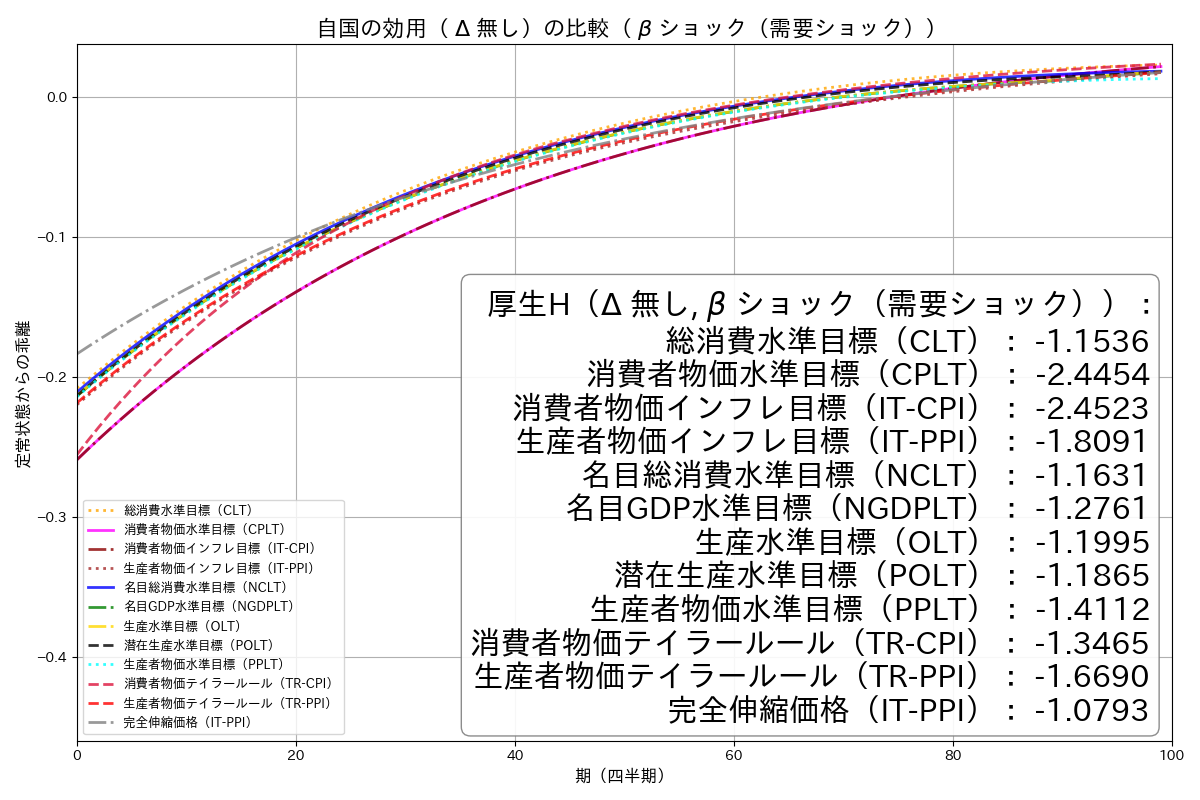
\includegraphics[width=0.9\textwidth]{comparison_graphs/beta_shock/beta_shock_utility_H_without_delta.png}
    \caption{自国の効用\(u^H\)と厚生\(W^H\)（\(\Delta\)無し）}
    \label{fig:chapter5_beta_shock_welfare_utility_H_without_Delta}
\end{figure}
\begin{figure}[H]
    \centering
    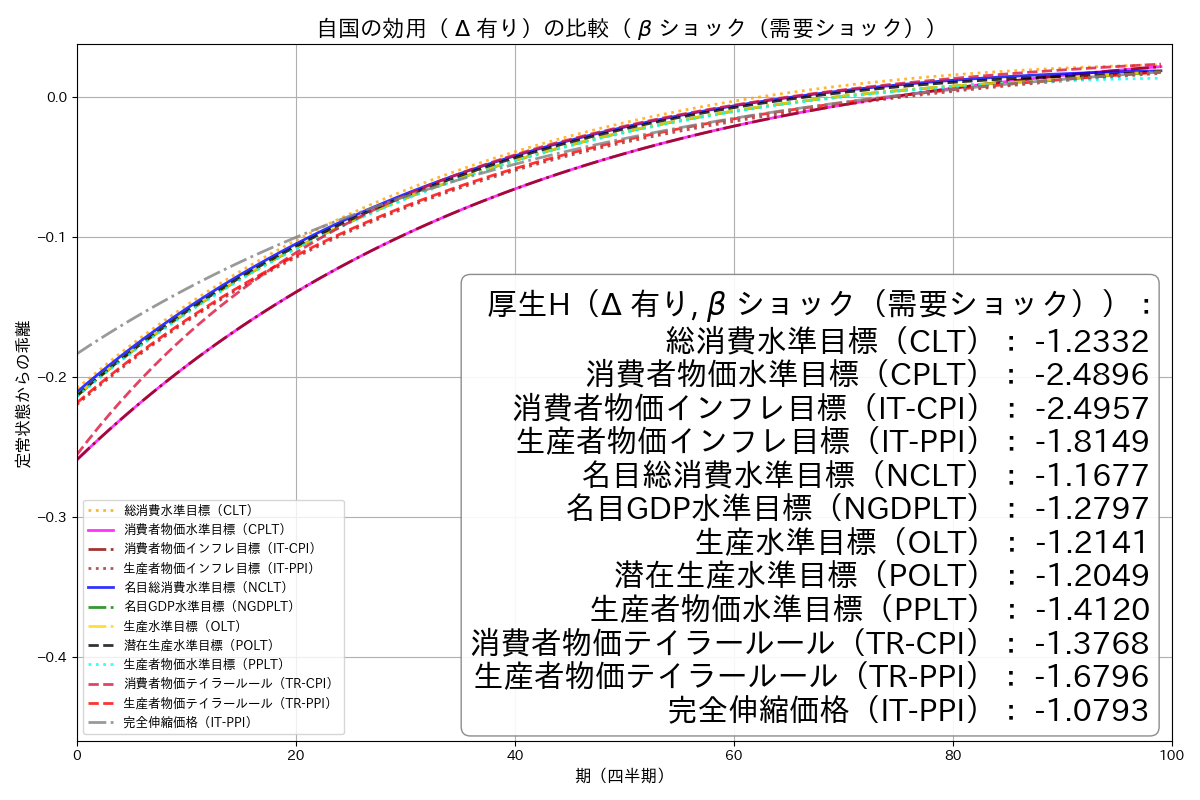
\includegraphics[width=0.9\textwidth]{comparison_graphs/beta_shock/beta_shock_utility_H_with_delta.png}
    \caption{自国の効用\(u^H\)と厚生\(W^H\)（\(\Delta\)有り）}
    \label{fig:chapter5_beta_shock_welfare_utility_H_with_Delta}
\end{figure}
\begin{figure}[H]
    \centering
    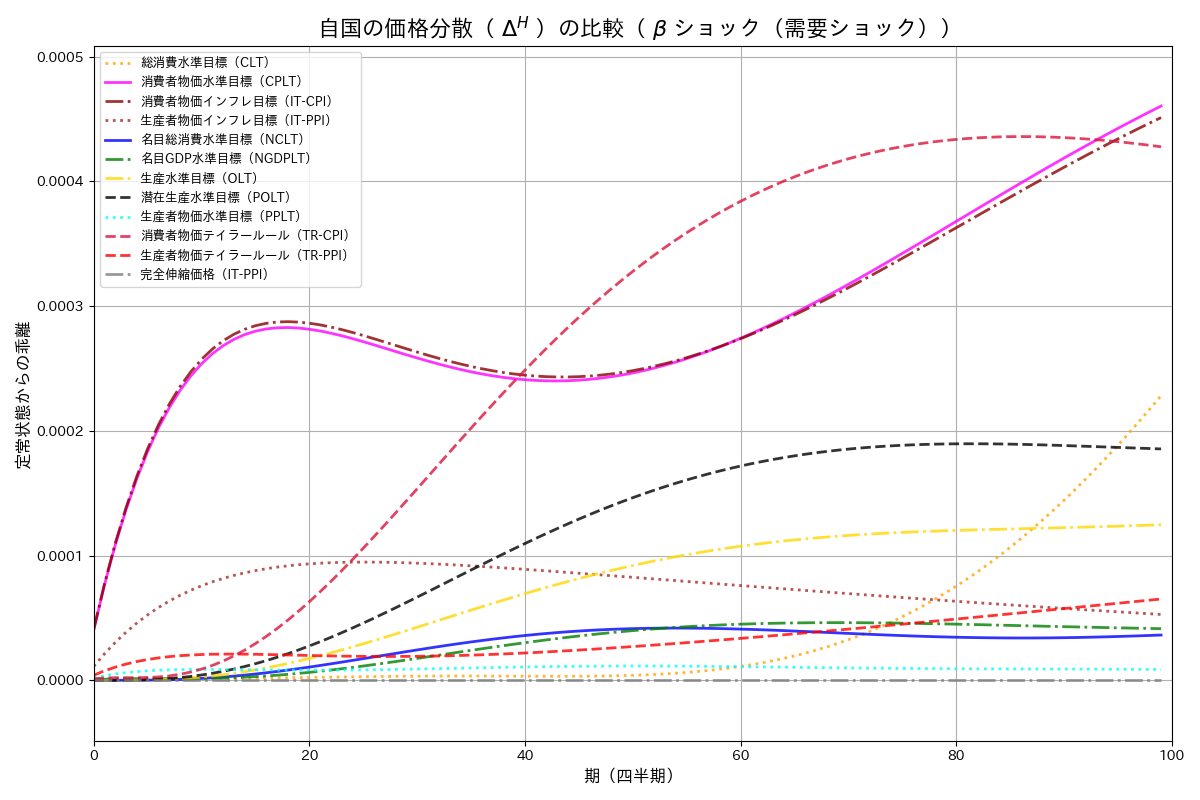
\includegraphics[width=0.9\textwidth]{comparison_graphs/beta_shock/beta_shock_Delta_H.png}
    \caption{自国の価格分散\(\Delta^H\)}
    \label{fig:chapter5_beta_shock_welfare_Delta_H}
\end{figure}

\paragraph{価格分散\(\Delta_t^H\)による厚生損失の比較}
\label{sec:chapter5_beta_shock_Delta_loss_comparison}
図
\ref{fig:chapter5_beta_shock_welfare_utility_H_without_Delta}
（\(\Delta_t^H\)無し）と図
\ref{fig:chapter5_beta_shock_welfare_utility_H_with_Delta}
（\(\Delta_t^H\)有り）を比較すると、
価格分散\(\Delta_t^H\)の導入が各政策の評価にどのような影響を与えるかがわかる。
この導入による厚生\(W_s^H\)の下落幅の大きい順に政策を示す。
\begin{table}[H]
\centering
\caption{価格分散に\(\Delta_t^H\)よる厚生損失の比較}
\label{tab:chapter5_beta_shock_welfare_Delta_comparison}
\begin{tabular}{lccc}
\hline
金融政策 & \(W_s^H\)（\(\Delta_t^H\)無し） & \(W_s^H\)（\(\Delta_t^H\)有り） & 下落幅（損失） \\
\hline
実質消費水準目標（CLT） & $-1.1536$ & $-1.2332$ & 0.0796 \\
消費者物価水準目標（CPLT） & $-2.4454$ & $-2.4896$ & 0.0442 \\
消費者物価インフレ目標（IT-CPI） & $-2.4523$ & $-2.4957$ & 0.0434 \\
消費者物価テイラールール（TR-CPI） & $-1.3465$ & $-1.3768$ & 0.0303 \\
潜在生産水準目標（POLT） & $-1.1865$ & $-1.2049$ & 0.0184 \\
生産水準目標（OLT） & $-1.1995$ & $-1.2141$ & 0.0146 \\
生産者物価テイラールール（TR-PPI） & $-1.6690$ & $-1.6796$ & 0.0106 \\
生産者物価インフレ目標（IT-PPI） & $-1.8091$ & $-1.8149$ & 0.0058 \\
名目総消費水準目標（NCLT） & $-1.1631$ & $-1.1677$ & 0.0046 \\
名目GDP水準目標（NGDPLT） & $-1.2761$ & $-1.2797$ & 0.0036 \\
生産者物価水準目標（PPLT） & $-1.4112$ & $-1.4120$ & 0.0008 \\
\hline
\end{tabular}
\end{table}
まずグラフや表から読み取れるように、
すべての政策において\(\Delta_t^H\)無しの場合よりも\(\Delta_t^H\)有りの場合の方が厚生\(W_s^H\)が低下している。
これは価格分散の乖離\(\hat{\Delta}_t^H\)が定義上1以上の値をとり、式
\eqref{form:chapter3_representative_household_welfare_home_representative_W_H_def}
\eqref{form:chapter5_beta_shock_welfare_u_H_minus_u_H_ss_eq}
により、これが大きいほど厚生\(W_s^H\)が押し下げられることになるからである。

\paragraph{厚生損失の絶対水準の比較}
\label{sec:chapter5_beta_shock_welfare_comparison}
次に価格分散\(\Delta_t^H\)を考慮した場合を例として
どの政策が最も厚生\(W_s^H\)の下落を抑制できているかを確認する。
厚生\(W_s^H\)の大きい順に政策を示す。
\begin{table}[H]
\centering
\caption{厚生損失の絶対水準の比較}
\label{tab:chapter5_beta_shock_welfare_comparison_ranking}
\begin{tabular}{lc}
\hline
金融政策 & \(W_s^H\)（\(\Delta_t^H\)有り） \\
\hline
名目総消費水準目標（NCLT） & $-1.1677$ \\
潜在生産水準目標（POLT） & $-1.2049$ \\
生産水準目標（OLT） & $-1.2141$ \\
実質消費水準目標（CLT） & $-1.2332$ \\
名目GDP水準目標（NGDPLT） & $-1.2797$ \\
消費者物価テイラールール（TR-CPI） & $-1.3768$ \\
生産者物価水準目標（PPLT） & $-1.4120$ \\
生産者物価テイラールール（TR-PPI） & $-1.6796$ \\
生産者物価インフレ目標（IT-PPI） & $-1.8149$ \\
消費者物価水準目標（CPLT） & $-2.4896$ \\
消費者物価インフレ目標（IT-CPI） & $-2.4957$ \\
\hline
\end{tabular}
\end{table}
NCLTが最も高い厚生\(W_s^H\)を達成しており\(\beta\)ショックによる負の影響を最小限に留めていることがわかる。
一方で消費者物価指数（CPI）\(p_t^{H\to W}\)のみを目標に含むIT-CPIやCPLTは極めて低い評価となった。

\subsection{遮断効果}
\label{sec:chapter5_beta_shock_insulation}
次に国際的な波及効果について考察する。
本稿のシミュレーションにおいては自国の金融政策の違いが主要な外国関連変数
\(\{\lambda_t^{H/*},\lambda_t^{F/*},p_t^{F*},i_t^F,c_t^{H\to F},c_t^{F\to F},y_t^F,l_t^F,
\bar{p}_t^{F*},\pi_t^{F*},\widetilde{p}_t^{F*},v_t^F,w_t^F,t_t^{F*},b_t^H,\Delta_t^F\}\) 
にまったく影響を与えないという結果が得られた。
これは遮断効果として知られている\parencite{ColeObstfeld1991}。
ただし完全伸縮物価IT-PPIのみグラフが異なっており、
これは価格硬直性パラメータ\(\xi^H\)が異なるためである。
遮断効果の詳しい説明は付録
\ref{sec:appendix_insulation_effect_TODO}
に記す。
\begin{figure}[H]
    \centering
    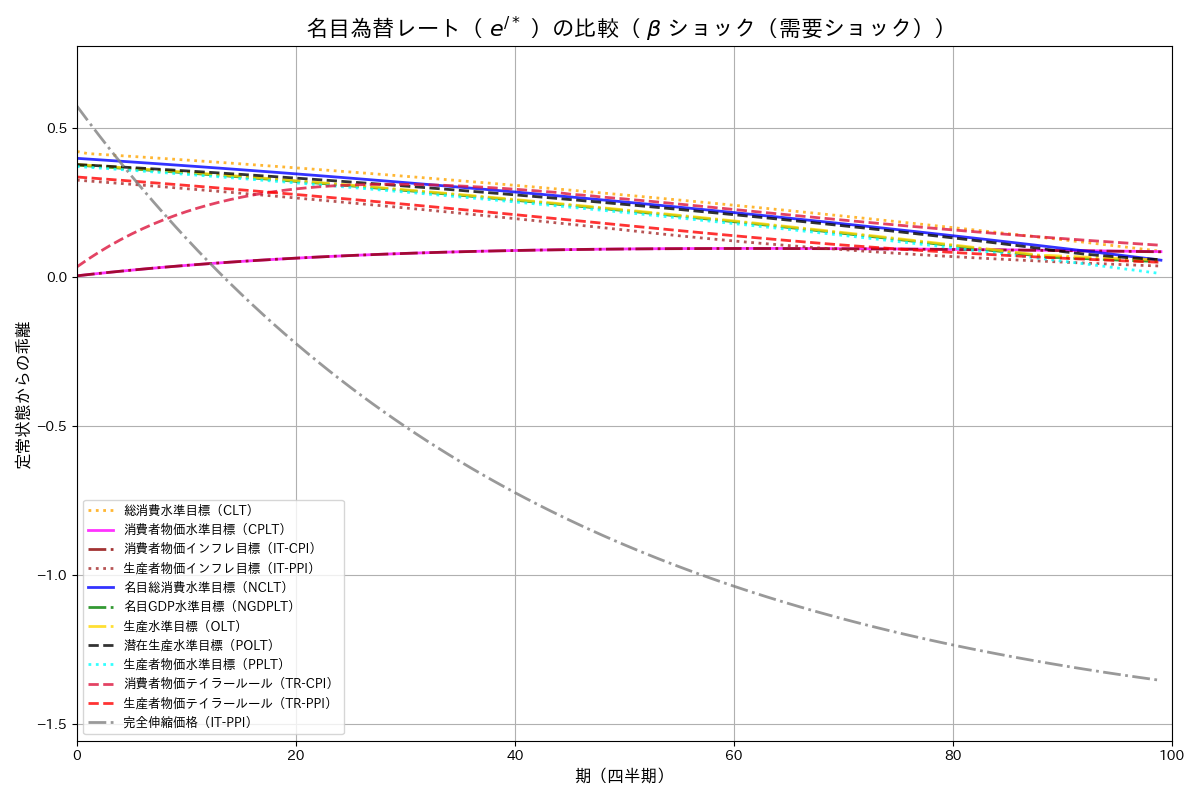
\includegraphics[width=0.9\textwidth]{comparison_graphs/beta_shock/beta_shock_e_slash_star.png}
    \caption{自国通貨建て名目為替レート（\(e^{/*}\)）}
    \label{fig:chapter5_beta_shock_insulation_e_slash_star}
\end{figure}
\begin{figure}[H]
    \centering
    \phantomcaption % 図番号を確保
    \label{fig:chapter5_beta_shock_foreign_vars}
    \makebox[\textwidth][c]{
        \begin{minipage}{1.2\textwidth}
            \centering
            \begin{subfigure}{0.48\linewidth}
                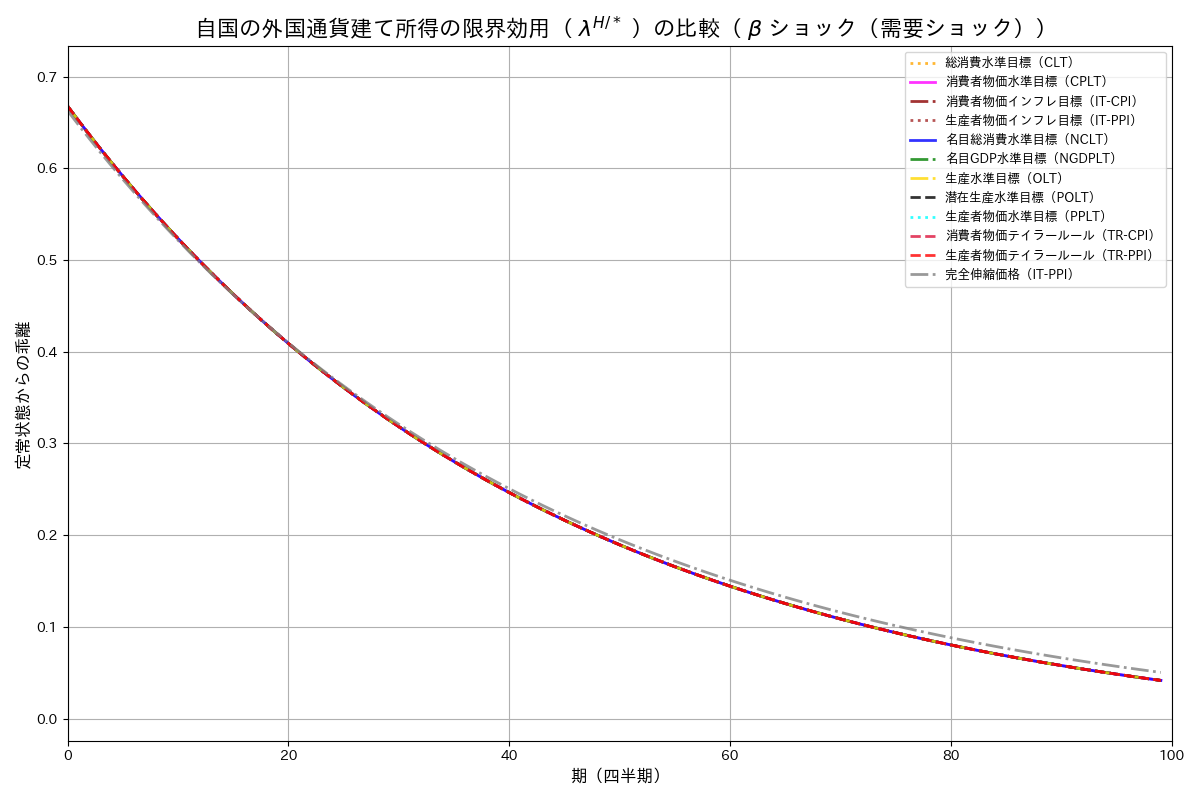
\includegraphics[width=\linewidth]{comparison_graphs/beta_shock/beta_shock_lambda_H_slash_star.png}
                \caption{自国の外国通貨建て所得の限界効用（\(\lambda^{H/*}\)）}
                \label{fig:chapter5_beta_shock_insulation_lambda_H_slash_star}
            \end{subfigure}
            \hfill
            \begin{subfigure}{0.48\linewidth}
                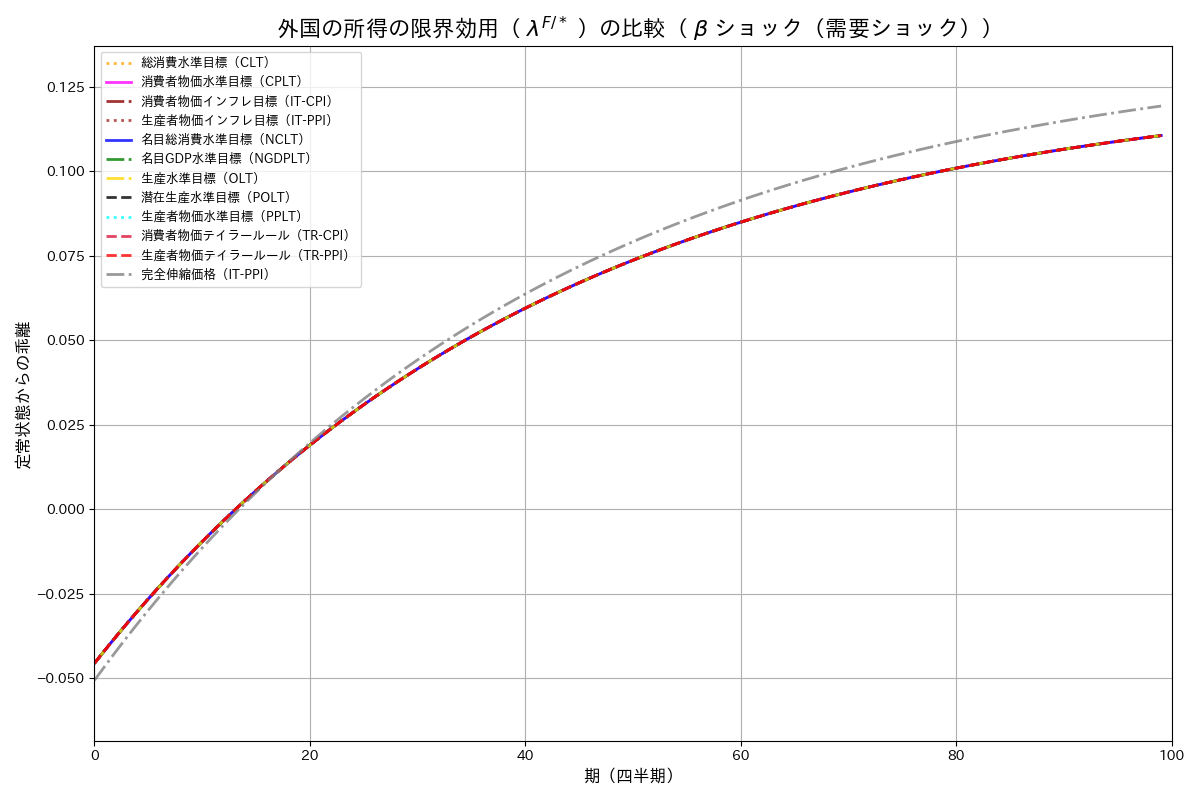
\includegraphics[width=\linewidth]{comparison_graphs/beta_shock/beta_shock_lambda_F_slash_star.png}
                \caption{外国の所得の限界効用（\(\lambda^{F/*}\)）}
                \label{fig:chapter5_beta_shock_insulation_lambda_F_slash_star}
            \end{subfigure}
        \end{minipage}
    }
\end{figure}
\begin{figure}[H]
    \ContinuedFloat
    \centering
    \makebox[\textwidth][c]{
        \begin{minipage}{1.2\textwidth}
            \centering
            \begin{subfigure}{0.48\linewidth}
                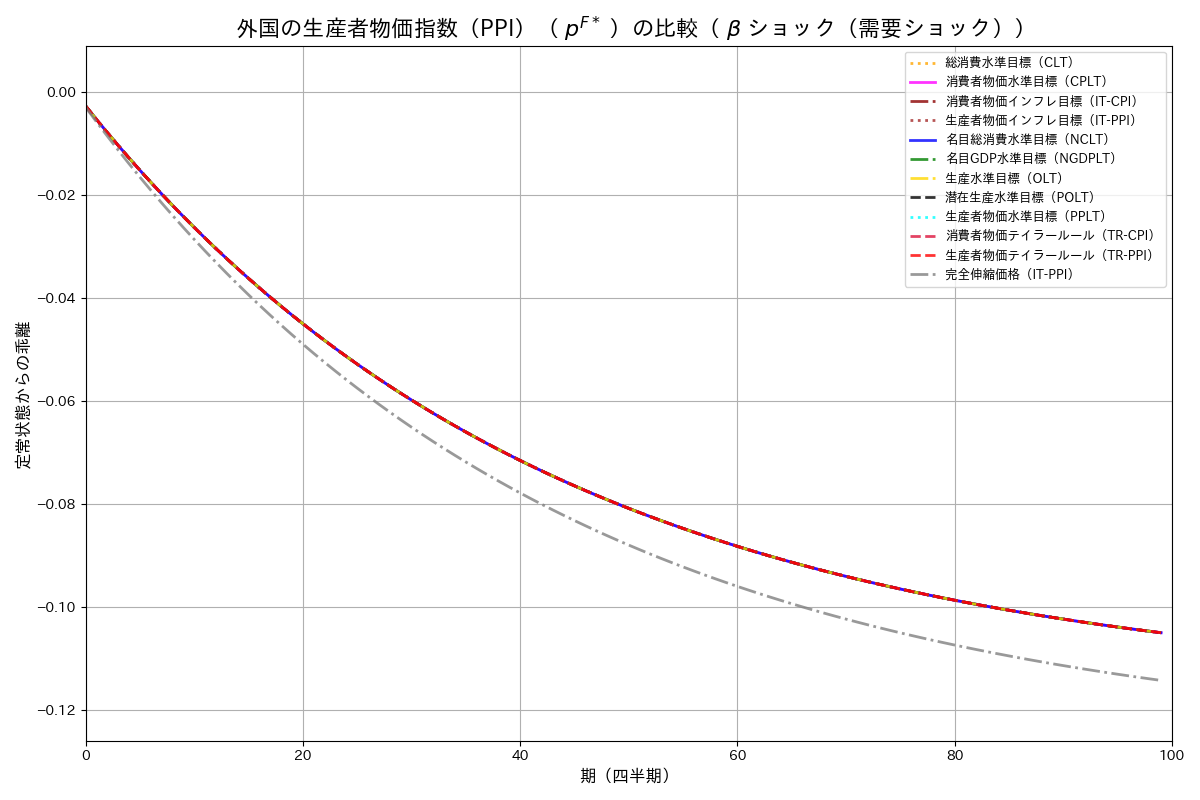
\includegraphics[width=\linewidth]{comparison_graphs/beta_shock/beta_shock_p_F_star.png}
                \caption{外国の生産者物価指数(PPI)（\(p^{F*}\)）}
                \label{fig:chapter5_beta_shock_insulation_p_F_star}
            \end{subfigure}
            \hfill
            \begin{subfigure}{0.48\linewidth}
                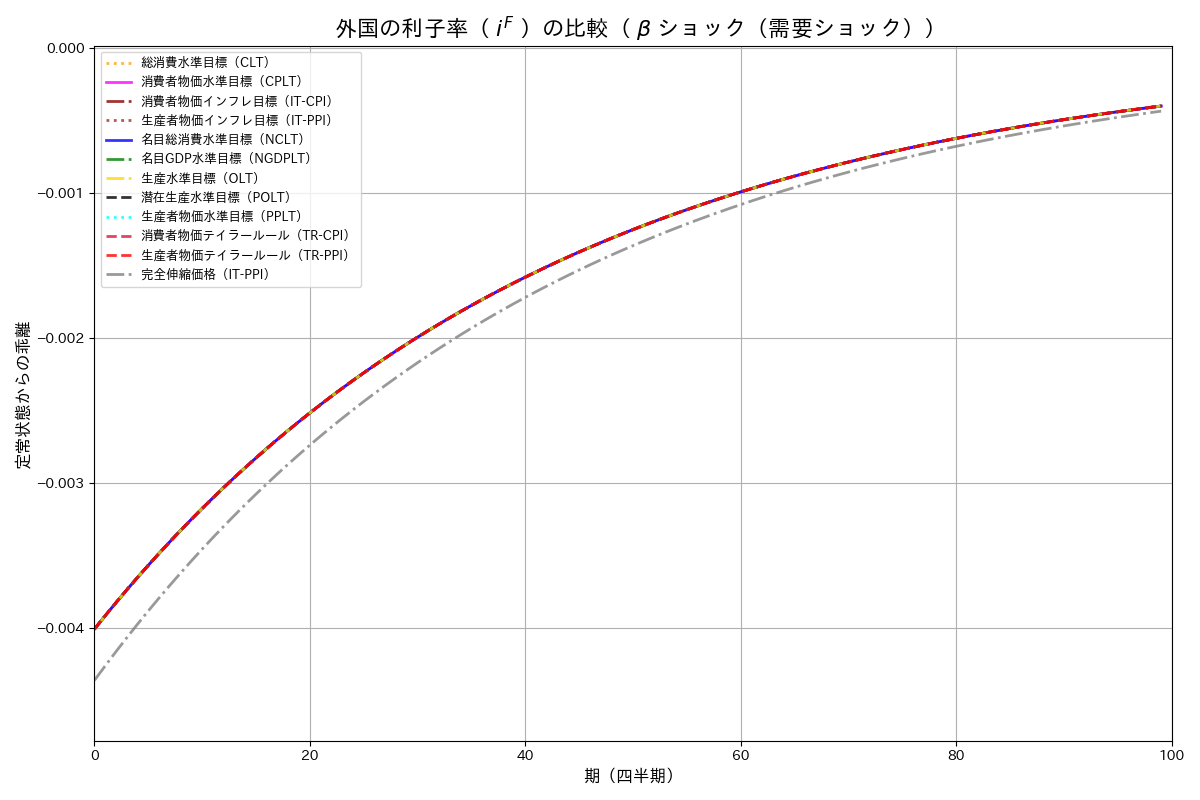
\includegraphics[width=\linewidth]{comparison_graphs/beta_shock/beta_shock_i_F.png}
                \caption{外国の名目利子率（\(i^F\)）}
                \label{fig:chapter5_beta_shock_insulation_i_F}
            \end{subfigure}
        \end{minipage}
    }
\end{figure}
\begin{figure}[H]
    \ContinuedFloat
    \centering
    \makebox[\textwidth][c]{
        \begin{minipage}{1.2\textwidth}
            \centering
            \begin{subfigure}{0.48\linewidth}
                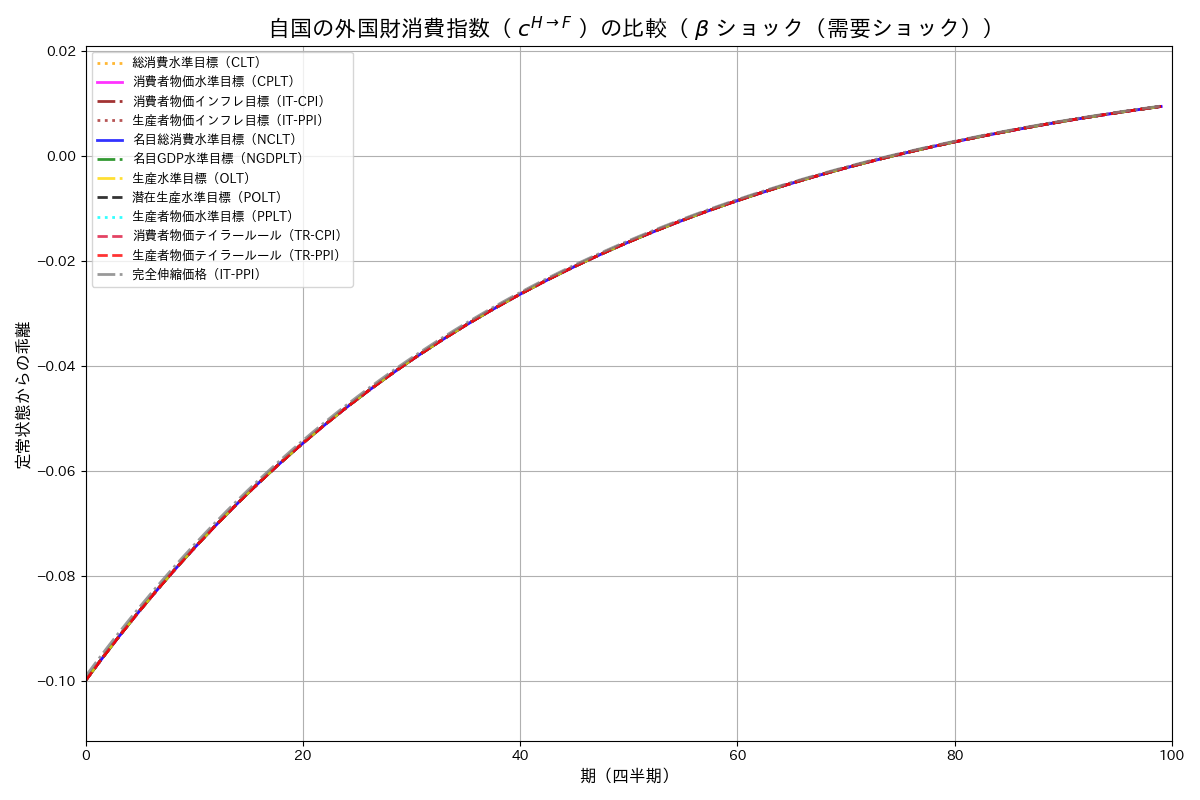
\includegraphics[width=\linewidth]{comparison_graphs/beta_shock/beta_shock_c_H_F.png}
                \caption{自国の外国財消費指数（\(c^{H\to F}\)）}
                \label{fig:chapter5_beta_shock_insulation_c_H_F}
            \end{subfigure}
            \hfill
            \begin{subfigure}{0.48\linewidth}
                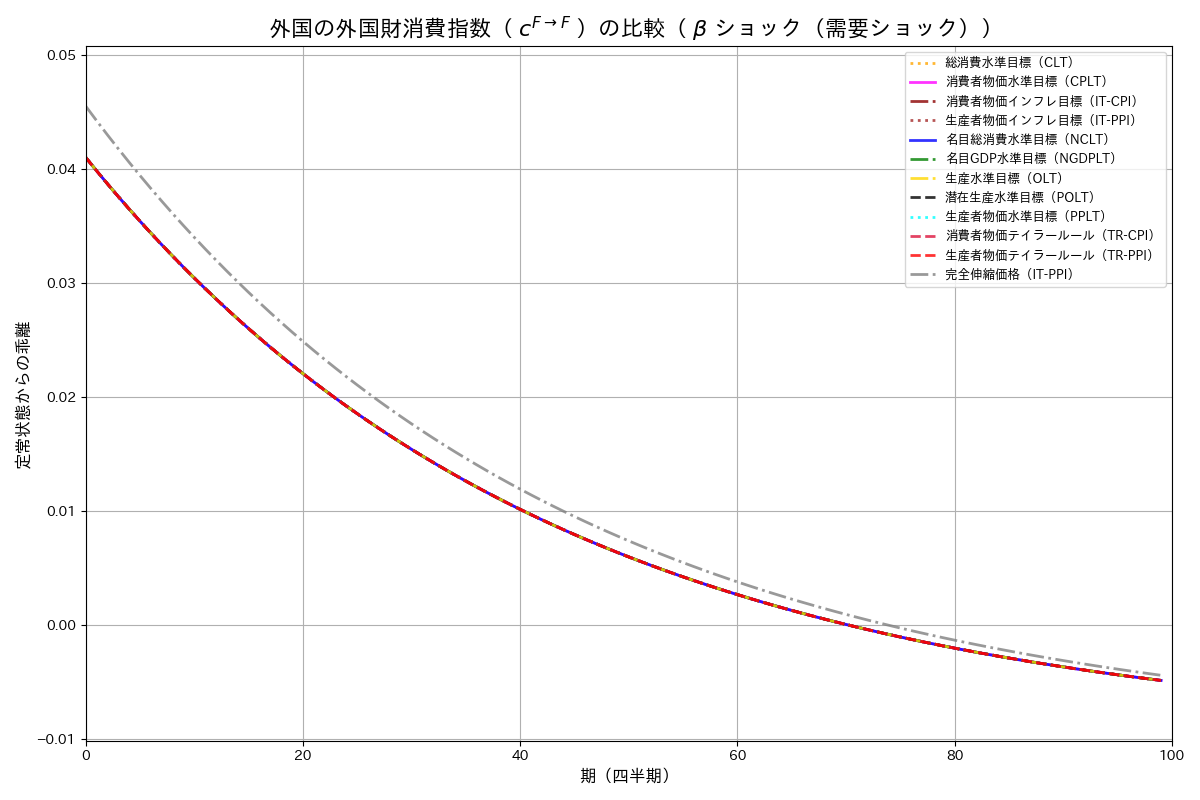
\includegraphics[width=\linewidth]{comparison_graphs/beta_shock/beta_shock_c_F_F.png}
                \caption{外国の外国財消費指数（\(c^{F\to F}\)）}
                \label{fig:chapter5_beta_shock_insulation_c_F_F}
            \end{subfigure}
        \end{minipage}
    }
\end{figure}
\begin{figure}[H]
    \ContinuedFloat
    \centering
    \makebox[\textwidth][c]{
        \begin{minipage}{1.2\textwidth}
            \centering
            \begin{subfigure}{0.48\linewidth}
                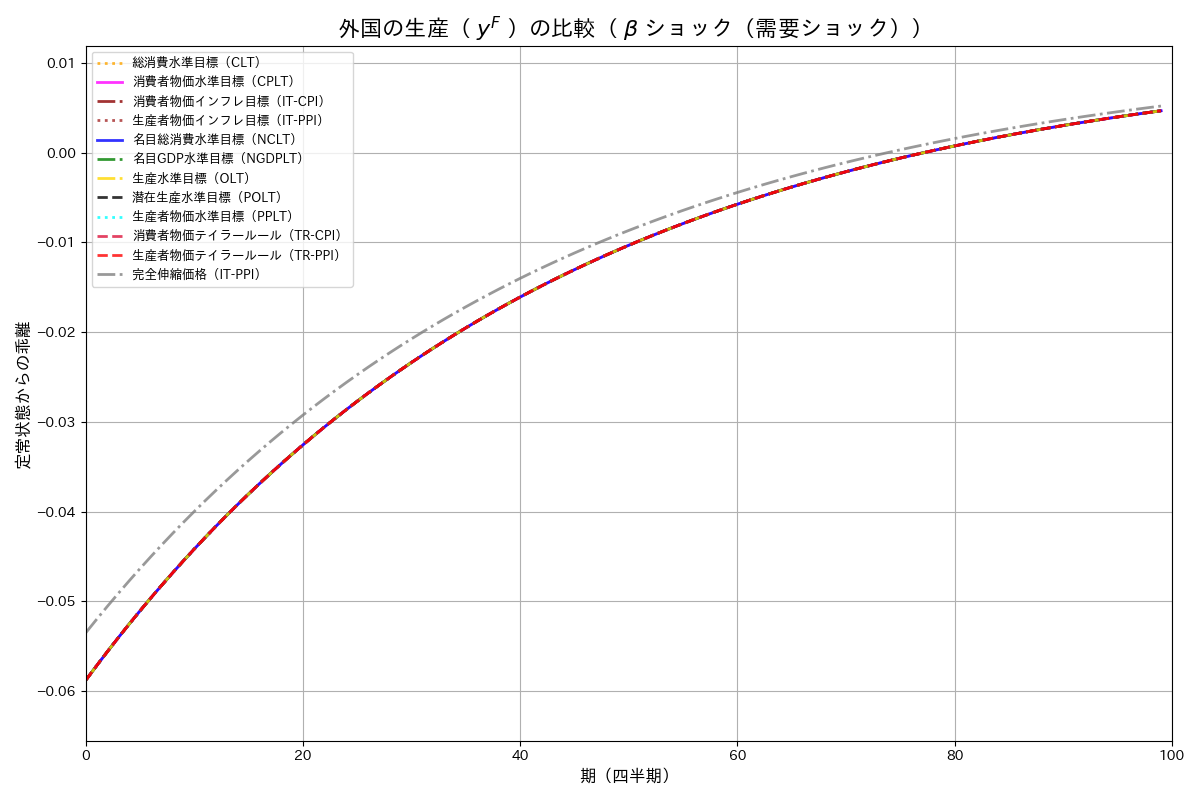
\includegraphics[width=\linewidth]{comparison_graphs/beta_shock/beta_shock_y_F.png}
                \caption{外国の生産（\(y^F\)）}
                \label{fig:chapter5_beta_shock_insulation_y_F}
            \end{subfigure}
            \hfill
            \begin{subfigure}{0.48\linewidth}
                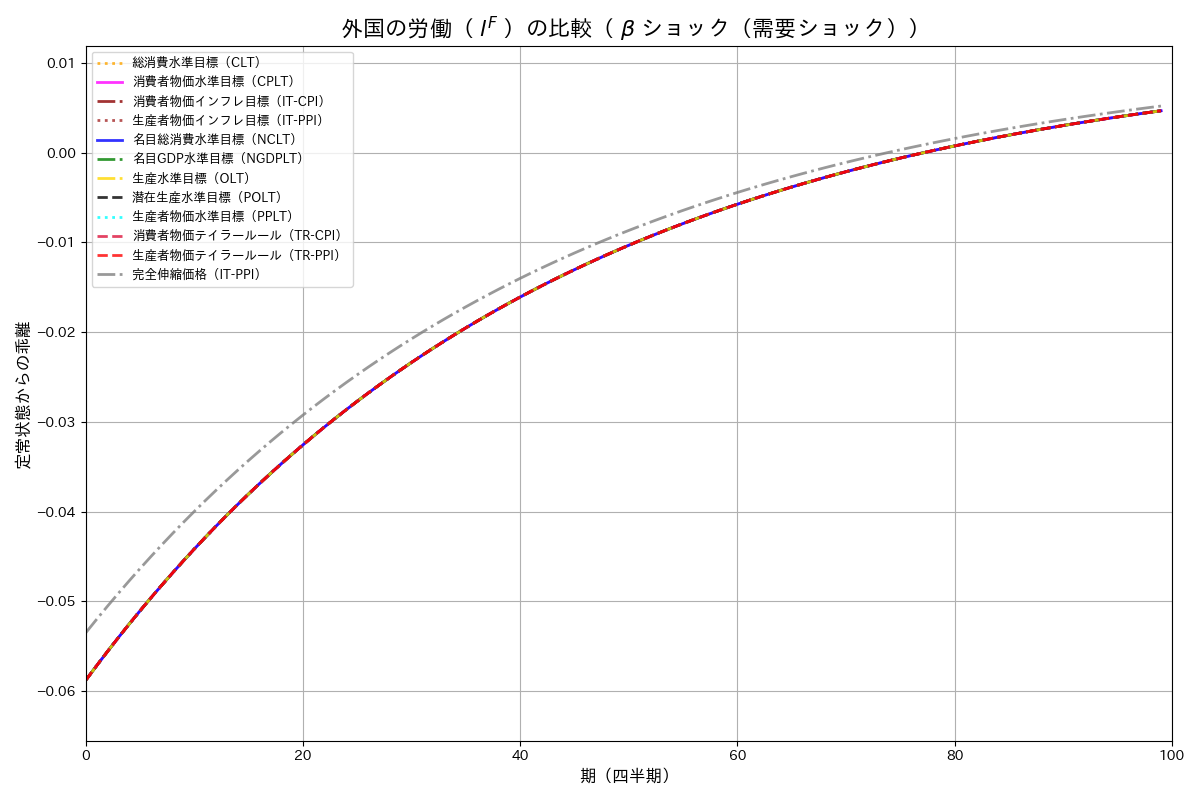
\includegraphics[width=\linewidth]{comparison_graphs/beta_shock/beta_shock_l_F.png}
                \caption{外国の労働（\(l^F\)）}
                \label{fig:chapter5_beta_shock_insulation_l_F}
            \end{subfigure}
        \end{minipage}
    }
\end{figure}
\begin{figure}[H]
    \ContinuedFloat
    \centering
    \makebox[\textwidth][c]{
        \begin{minipage}{1.2\textwidth}
            \centering
            \begin{subfigure}{0.48\linewidth}
                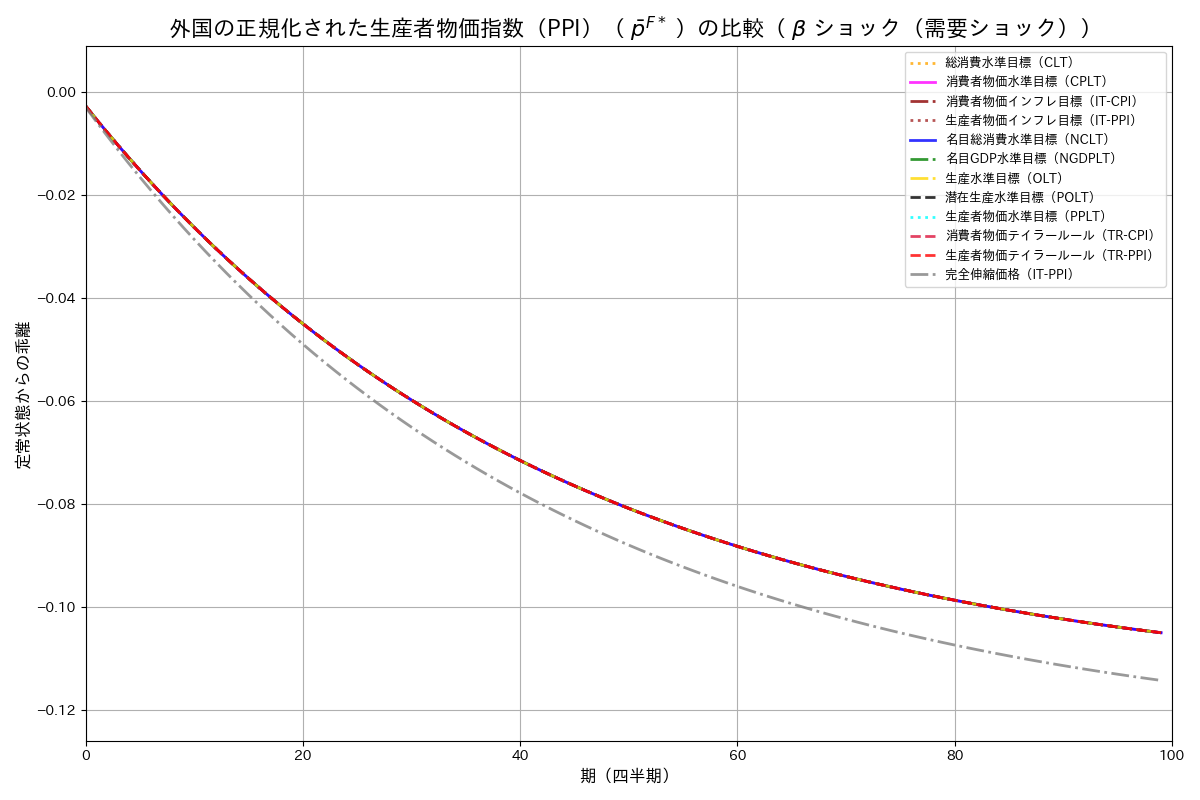
\includegraphics[width=\linewidth]{comparison_graphs/beta_shock/beta_shock_p_F_star_bar.png}
                \caption{外国の正規化された生産者物価指数(PPI)（\(\bar{p}^{F*}\)）}
                \label{fig:chapter5_beta_shock_insulation_p_F_star_bar}
            \end{subfigure}
            \hfill
            \begin{subfigure}{0.48\linewidth}
                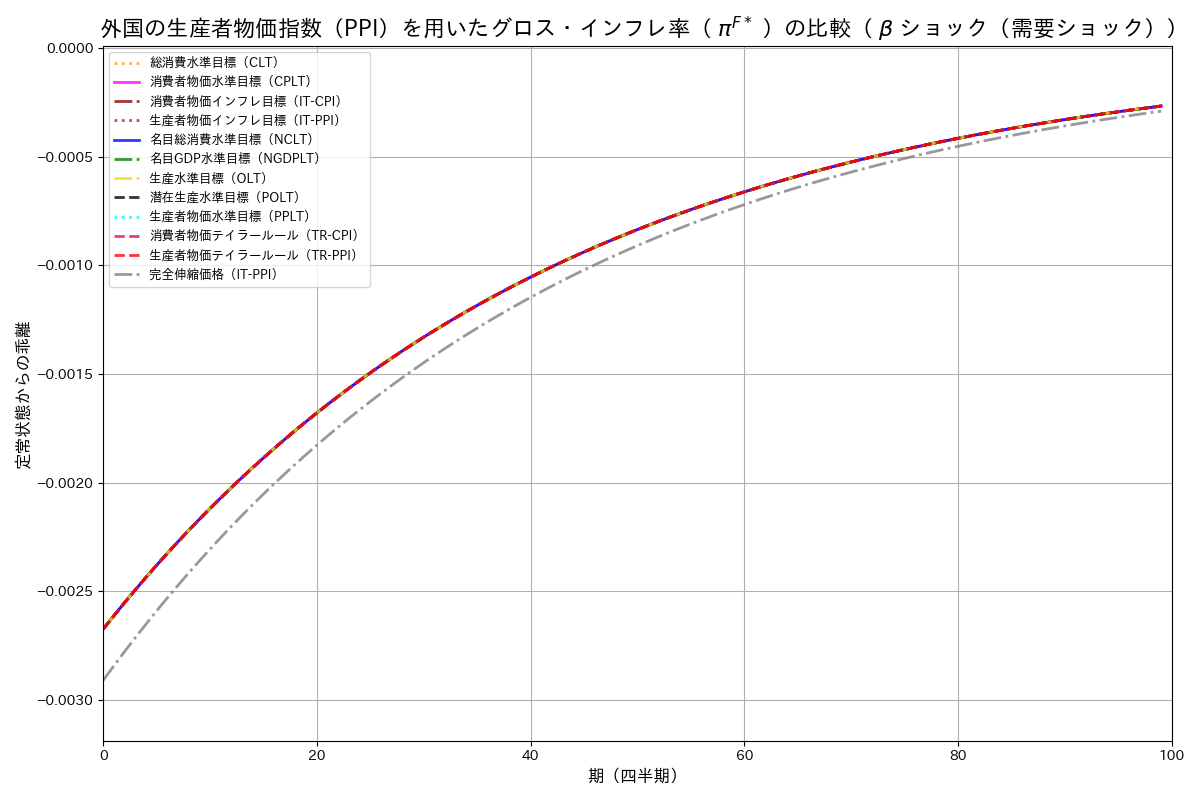
\includegraphics[width=\linewidth]{comparison_graphs/beta_shock/beta_shock_pi_F_star.png}
                \caption{外国の正規化された生産者物価指数(PPI)を用いたグロス・インフレ率（\(\pi^{F*}\)）}
                \label{fig:chapter5_beta_shock_insulation_pi_F_star}
            \end{subfigure}
        \end{minipage}
    }
\end{figure}
\begin{figure}[H]
    \ContinuedFloat
    \centering
    \makebox[\textwidth][c]{
        \begin{minipage}{1.2\textwidth}
            \centering
            \begin{subfigure}{0.48\linewidth}
                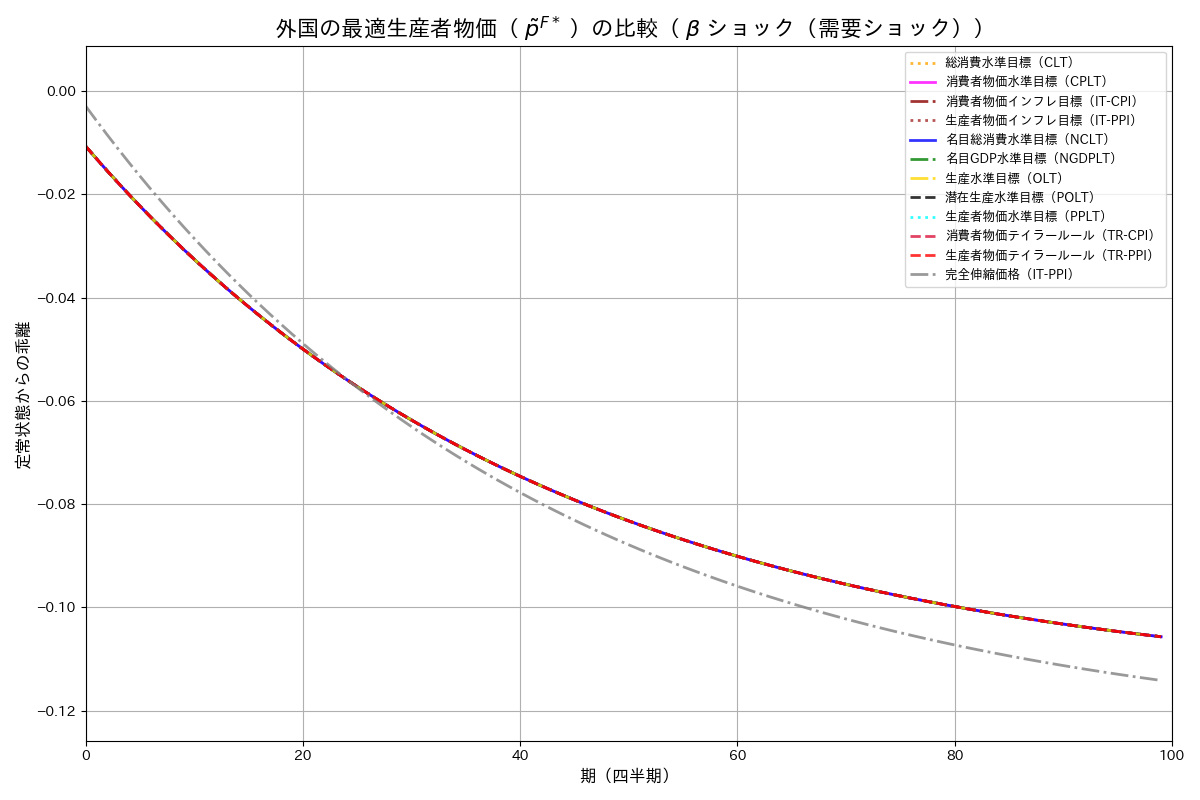
\includegraphics[width=\linewidth]{comparison_graphs/beta_shock/beta_shock_p_F_star_tilde.png}
                \caption{外国の最適生産者物価（\(\widetilde{p}^{F*}\)）}
                \label{fig:chapter5_beta_shock_insulation_p_F_star_tilde_sub}
            \end{subfigure}
            \hfill
            \begin{subfigure}{0.48\linewidth}
                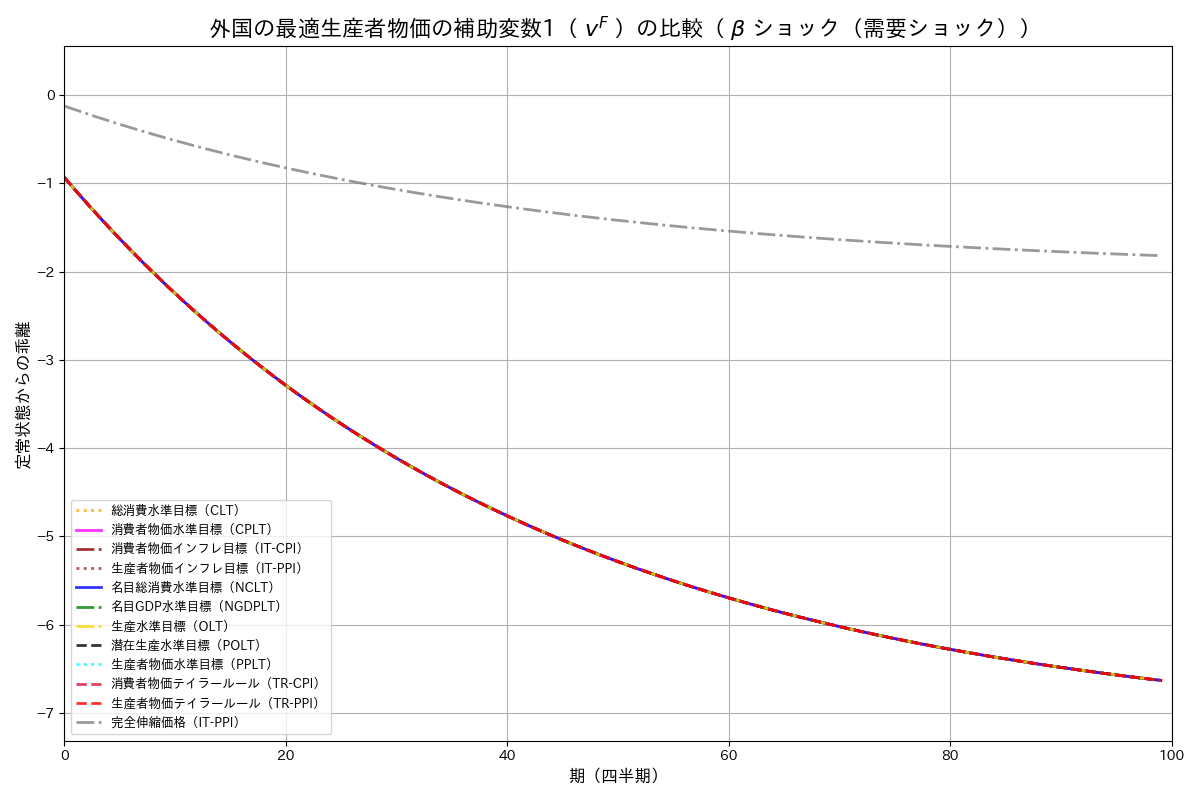
\includegraphics[width=\linewidth]{comparison_graphs/beta_shock/beta_shock_v_F.png}
                \caption{外国の最適生産者物価の補助変数1（\(v^F\)）}
                \label{fig:chapter5_beta_shock_insulation_v_F}
            \end{subfigure}
        \end{minipage}
    }
\end{figure}
\begin{figure}[H]
    \ContinuedFloat
    \centering
    \makebox[\textwidth][c]{
        \begin{minipage}{1.2\textwidth}
            \centering
            \begin{subfigure}{0.48\linewidth}
                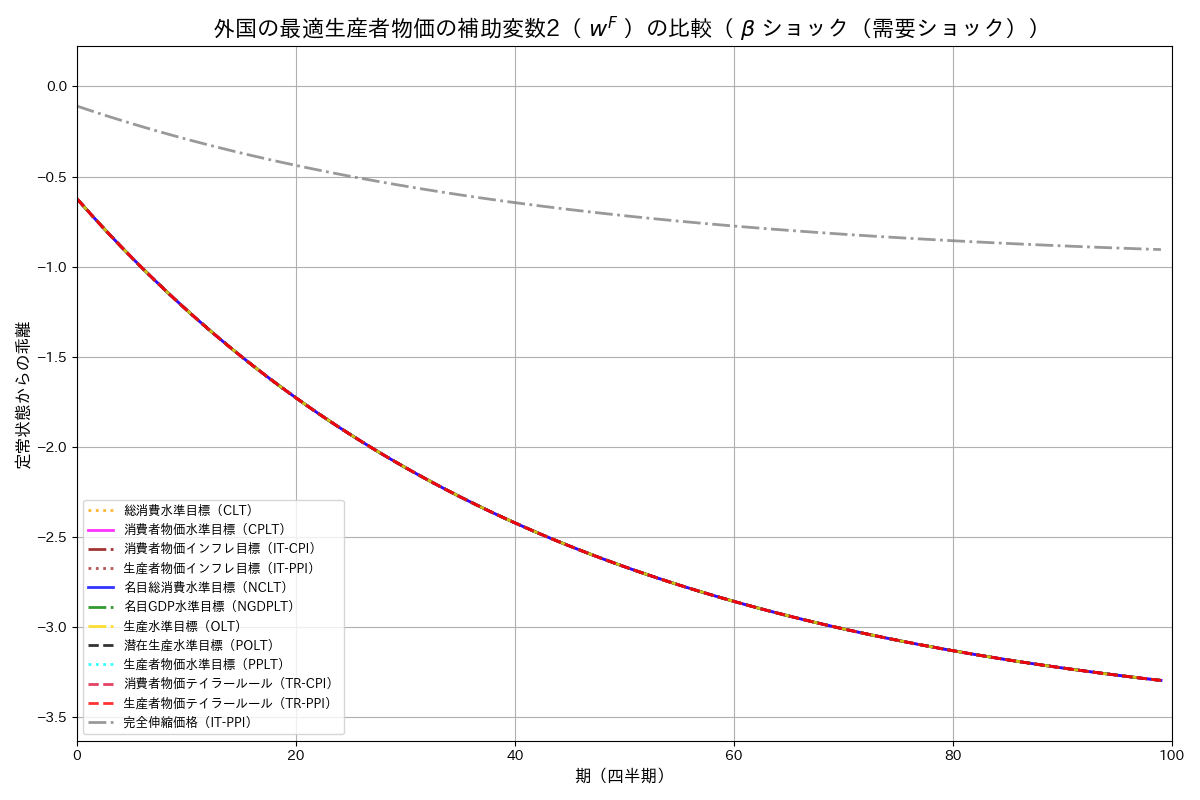
\includegraphics[width=\linewidth]{comparison_graphs/beta_shock/beta_shock_w_F.png}
                \caption{外国の最適生産者物価の補助変数2（\(w^F\)）}
                \label{fig:chapter5_beta_shock_insulation_w_F}
            \end{subfigure}
            \hfill
            \begin{subfigure}{0.48\linewidth}
                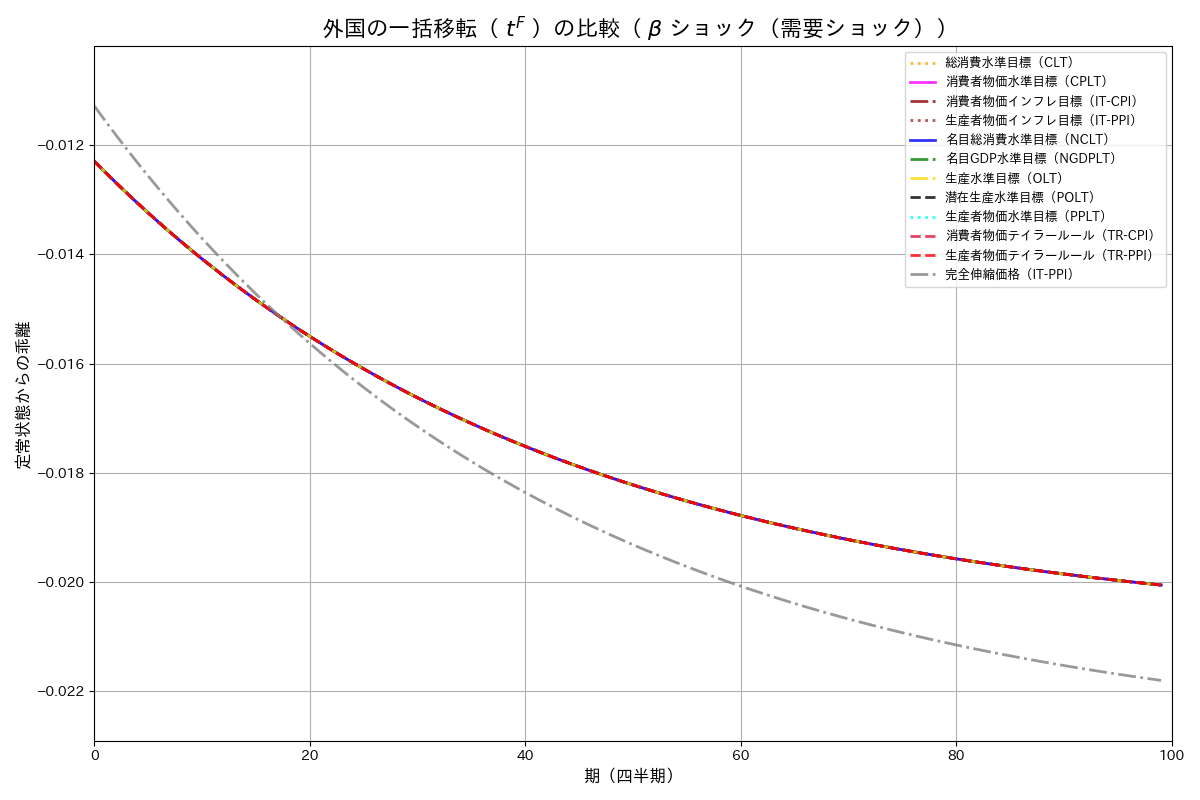
\includegraphics[width=\linewidth]{comparison_graphs/beta_shock/beta_shock_t_F.png}
                \caption{外国の一括移転（\(t^F\)）}
                \label{fig:chapter5_beta_shock_insulation_t_F}
            \end{subfigure}
        \end{minipage}
    }
\end{figure}
\begin{figure}[H]
    \ContinuedFloat
    \centering
    \makebox[\textwidth][c]{
        \begin{minipage}{1.2\textwidth}
            \centering
            \begin{subfigure}{0.48\linewidth}
                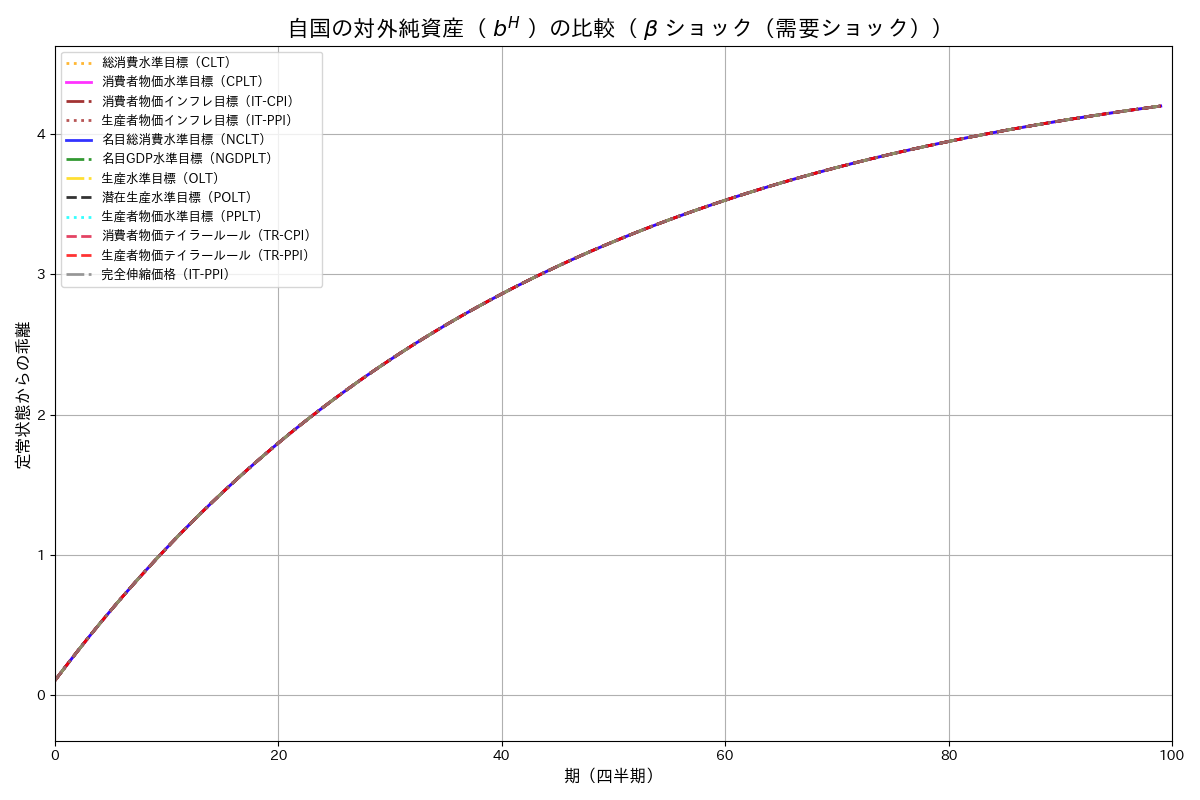
\includegraphics[width=\linewidth]{comparison_graphs/beta_shock/beta_shock_b_H.png}
                \caption{自国の対外純資産（\(b^H\)）}
                \label{fig:chapter5_beta_shock_insulation_b_H}
            \end{subfigure}
            \begin{subfigure}{0.48\linewidth}
                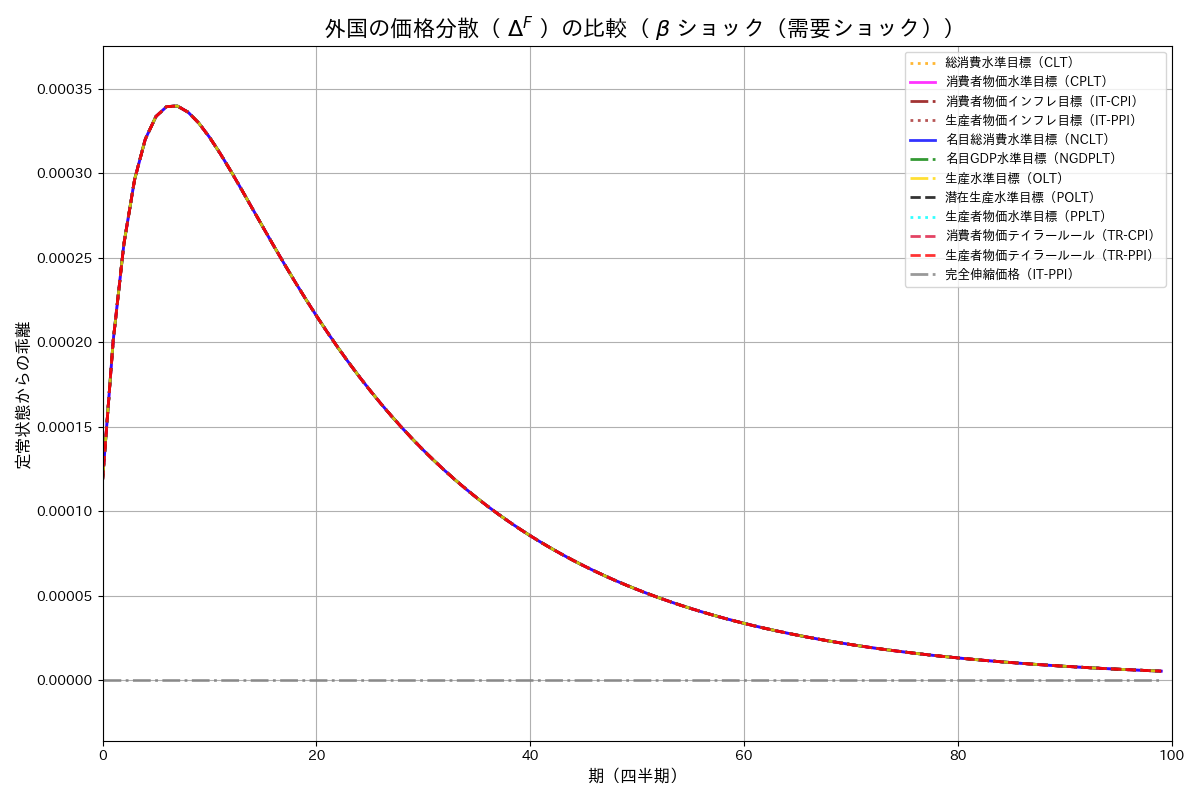
\includegraphics[width=\linewidth]{comparison_graphs/beta_shock/beta_shock_Delta_F.png}
                \caption{外国の価格分散（\(\Delta^F\)）}
                \label{fig:chapter5_beta_shock_insulation_Delta_F}
            \end{subfigure}
        \end{minipage}
    }
    % 最後にまとめてキャプションを表示
    \caption{外国経済変数のインパルス応答関数（全政策で不変）}
\end{figure}

\subsection{AS-AD分析}
\label{sec:chapter5_beta_shock_asad}

本節では効用や為替レートも含む主要な自国関連変数のグラフを掲載し、各金融政策についてその効果をAS-AD分析により解釈する。
\begin{figure}[H]
    \centering
    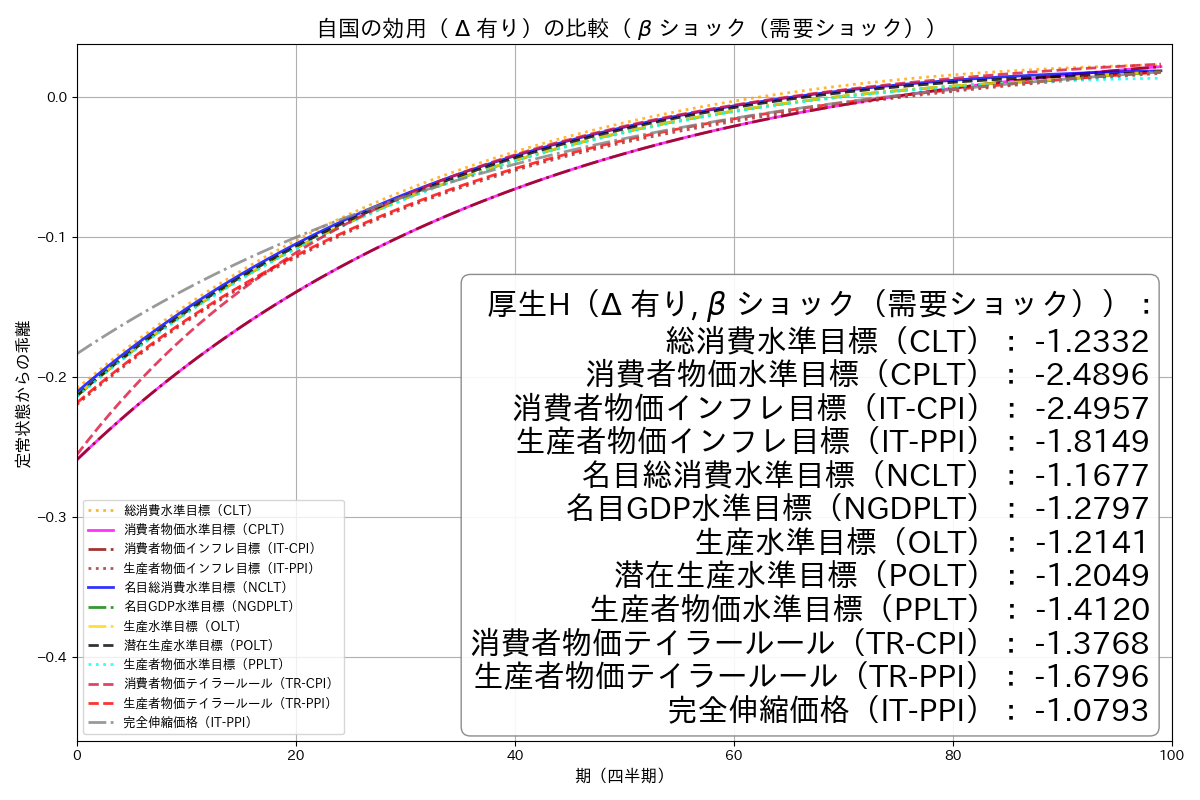
\includegraphics[width=0.9\textwidth]{comparison_graphs/beta_shock/beta_shock_utility_H_with_delta.png}
    \caption{自国の効用\(u^H\)と厚生\(W^H\)（\(\Delta\)有り）}
    \label{fig:chapter5_beta_shock_asad_utility_H_with_delta}
\end{figure}
\begin{figure}[H]
    \centering
    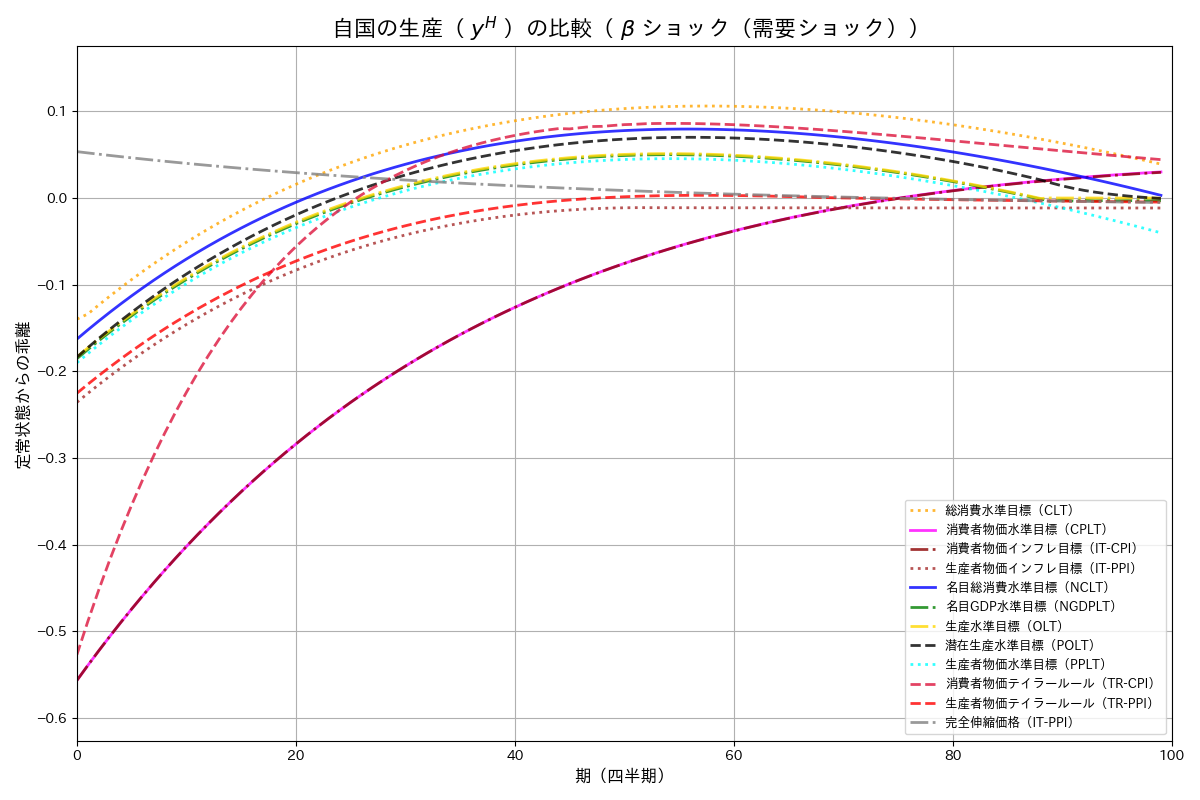
\includegraphics[width=0.9\textwidth]{comparison_graphs/beta_shock/beta_shock_y_H.png}
    \caption{自国の生産\(y^H\)}
    \label{fig:chapter5_beta_shock_asad_y_H}
\end{figure}
\begin{figure}[H]
    \centering
    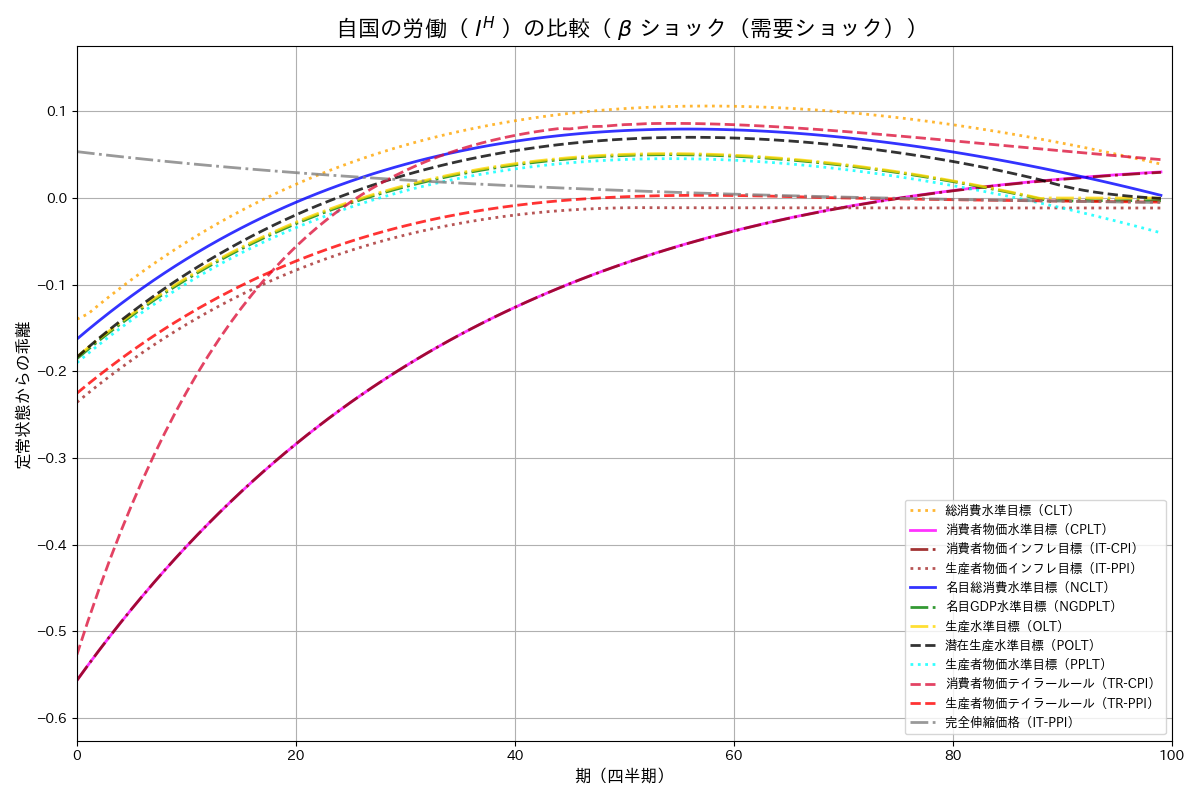
\includegraphics[width=0.9\textwidth]{comparison_graphs/beta_shock/beta_shock_l_H.png}
    \caption{自国の労働\(l^H\)}
    \label{fig:chapter5_beta_shock_asad_l_H}
\end{figure}
\begin{figure}[H]
    \centering
    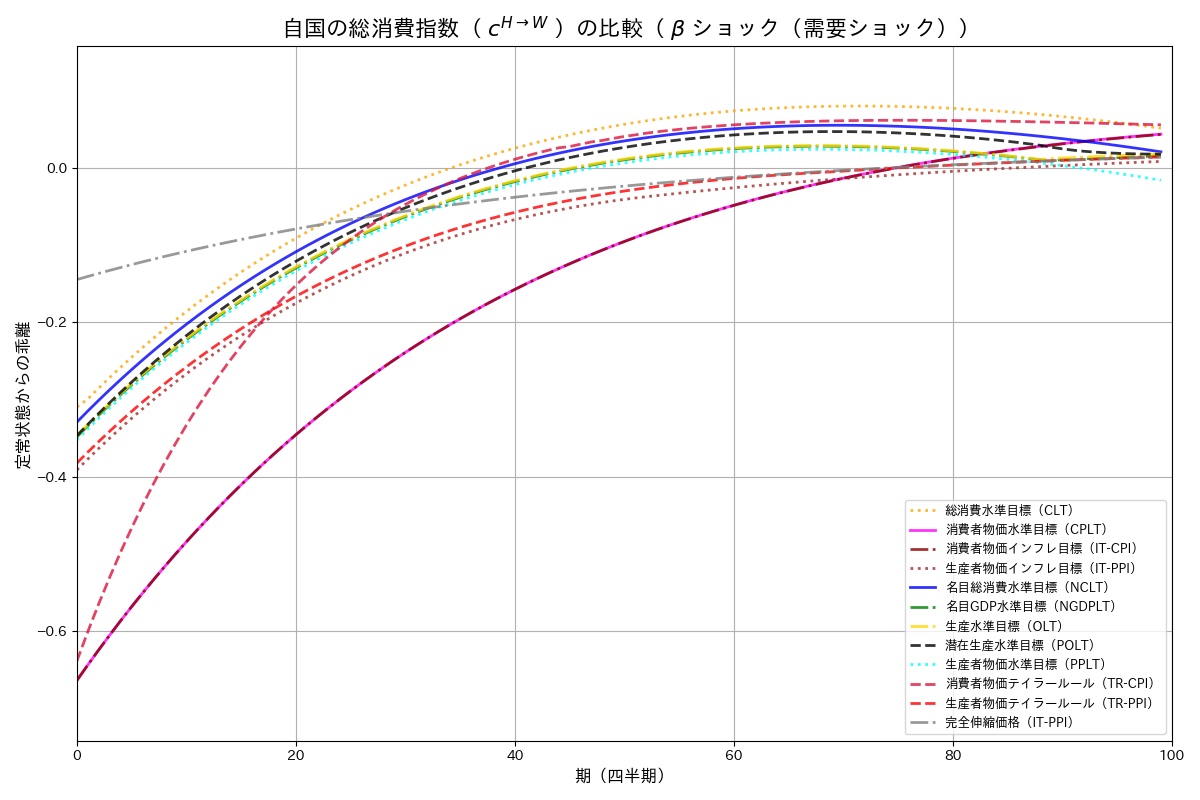
\includegraphics[width=0.9\textwidth]{comparison_graphs/beta_shock/beta_shock_c_H_W.png}
    \caption{自国の総消費指数\(c^{H\to W}\)}
    \label{fig:chapter5_beta_shock_asad_c_H_W}
\end{figure}
\begin{figure}[H]
    \centering
    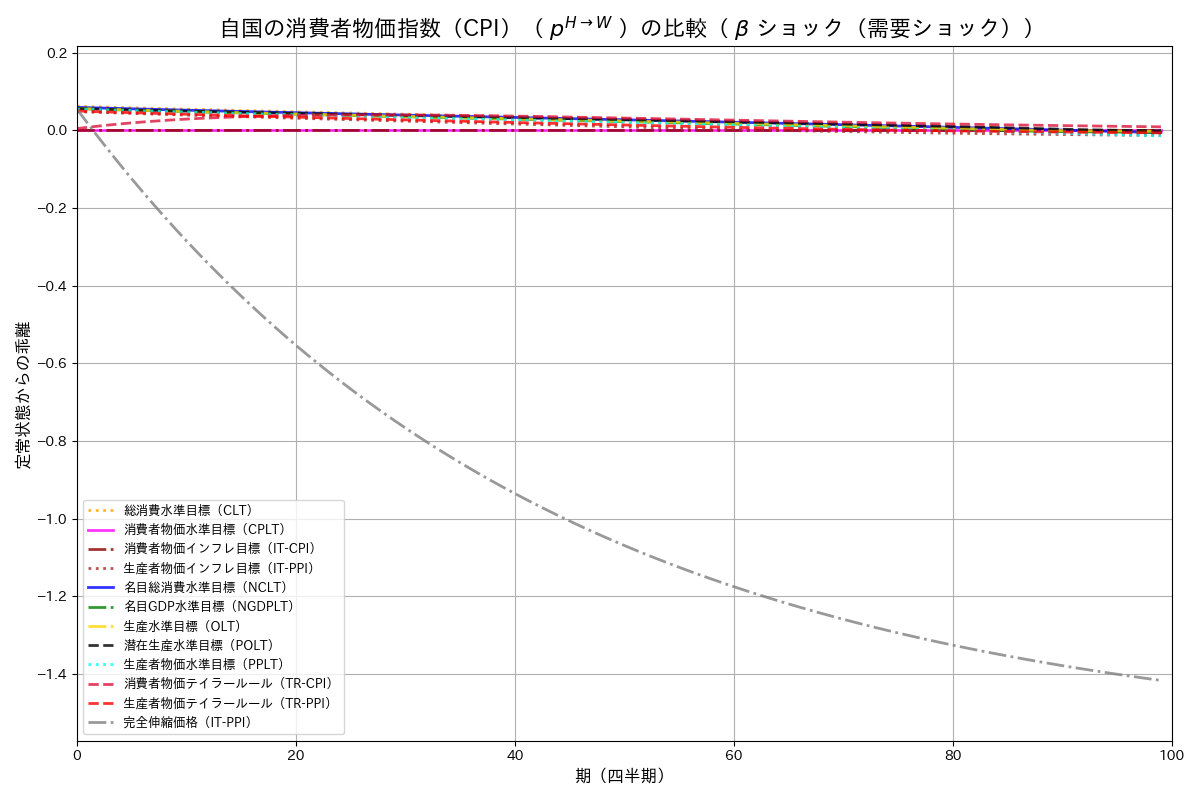
\includegraphics[width=0.9\textwidth]{comparison_graphs/beta_shock/beta_shock_p_H_W.png}
    \caption{自国の消費者物価指数\(p^{H\to W}\)}
    \label{fig:chapter5_beta_shock_asad_p_H_W}
\end{figure}
\begin{figure}[H]
    \centering
    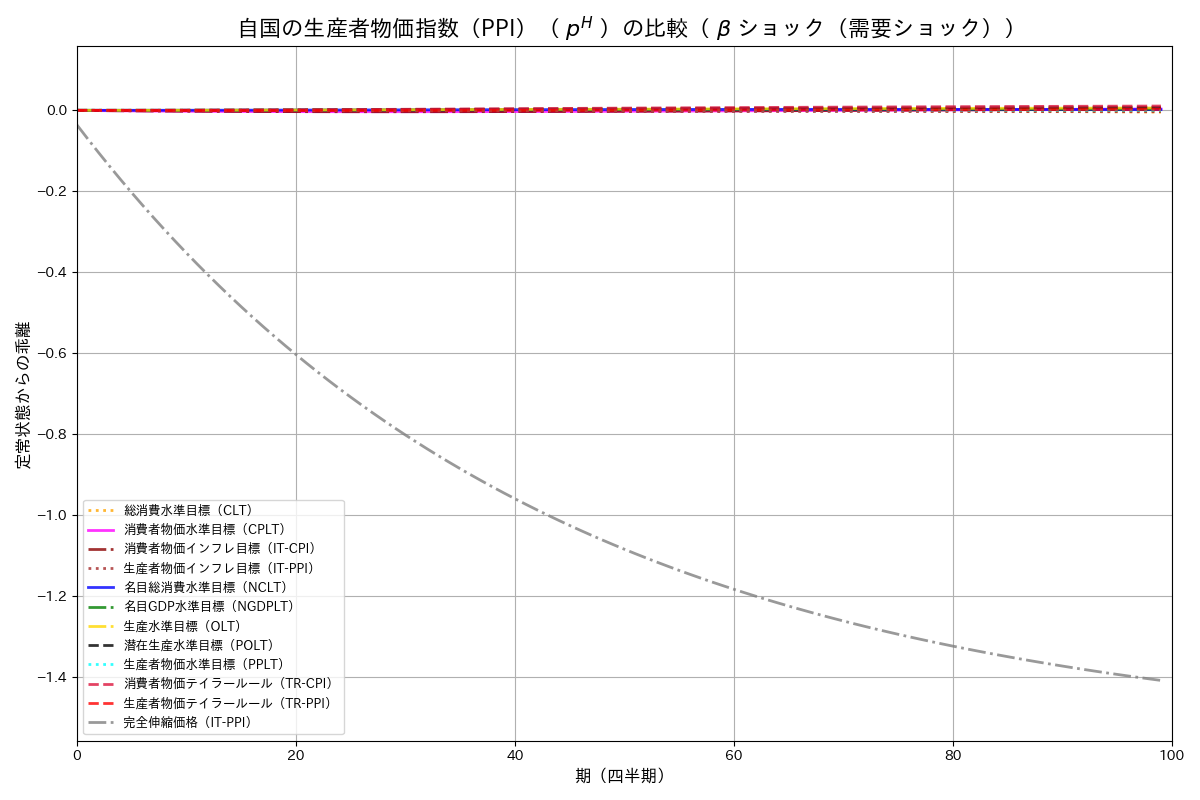
\includegraphics[width=0.9\textwidth]{comparison_graphs/beta_shock/beta_shock_p_H.png}
    \caption{自国の生産者物価指数PPI\(p^H\)}
    \label{fig:chapter5_beta_shock_asad_p_H}
\end{figure}
\begin{figure}[H]
    \centering
    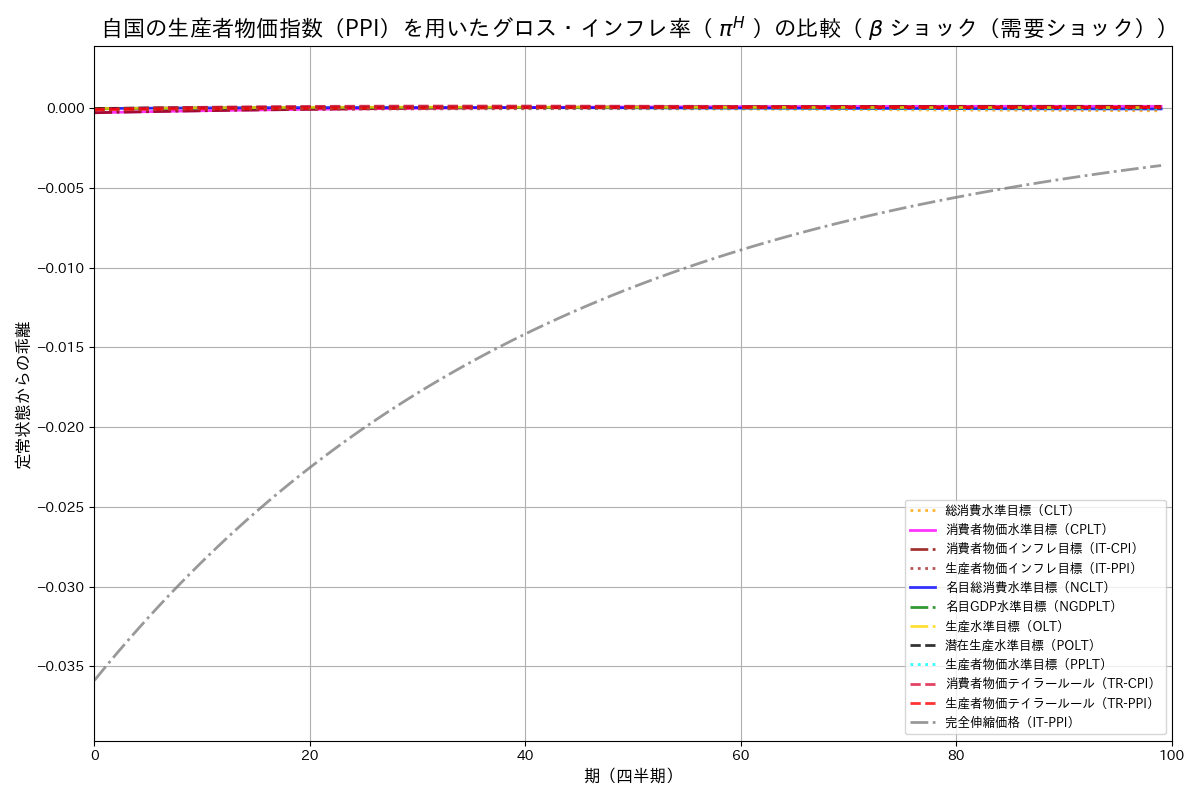
\includegraphics[width=0.9\textwidth]{comparison_graphs/beta_shock/beta_shock_pi_H.png}
    \caption{自国の生産者物価指数PPIを用いたグロス・インフレ率\(\pi^H\)}
    \label{fig:chapter5_beta_shock_asad_pi_H}
\end{figure}
\begin{figure}[H]
    \centering
    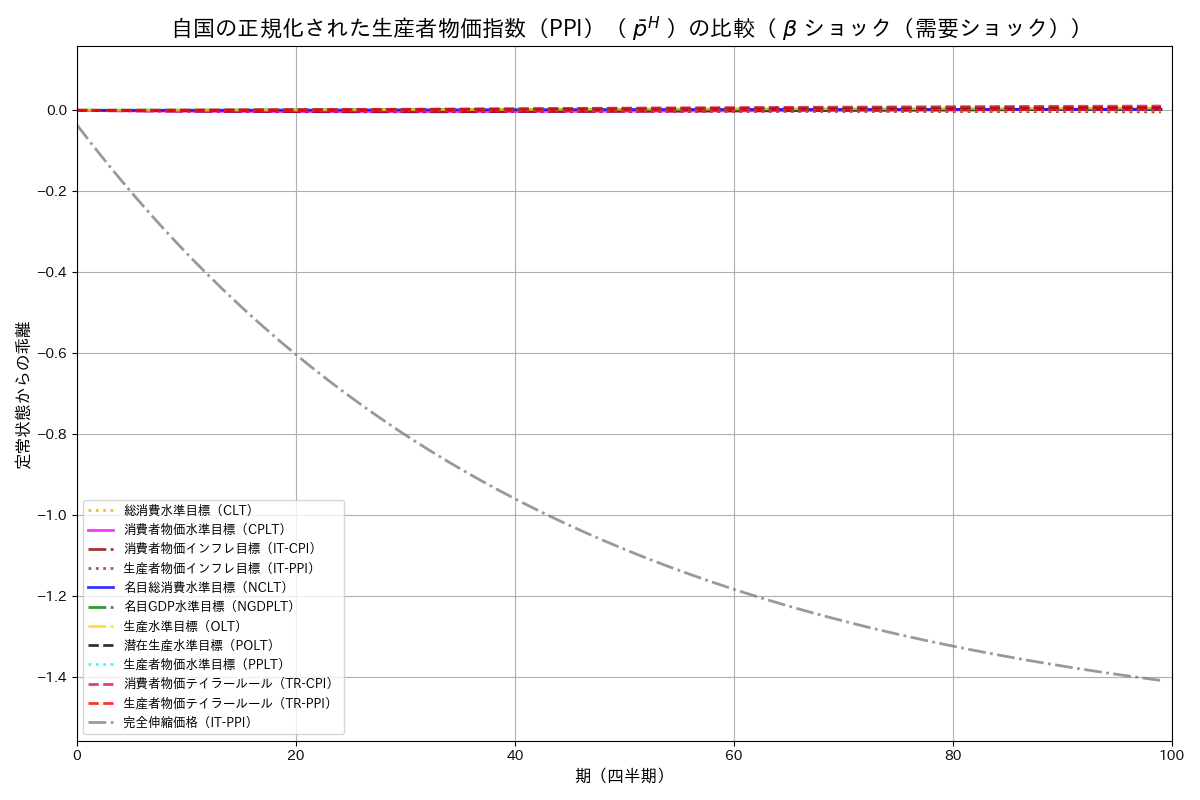
\includegraphics[width=0.9\textwidth]{comparison_graphs/beta_shock/beta_shock_p_H_bar.png}
    \caption{自国の正規化された生産者物価指数PPI\(\bar{p}^H\)}
    \label{fig:chapter5_beta_shock_asad_p_H_bar}
\end{figure}
\begin{figure}[H]
    \centering
    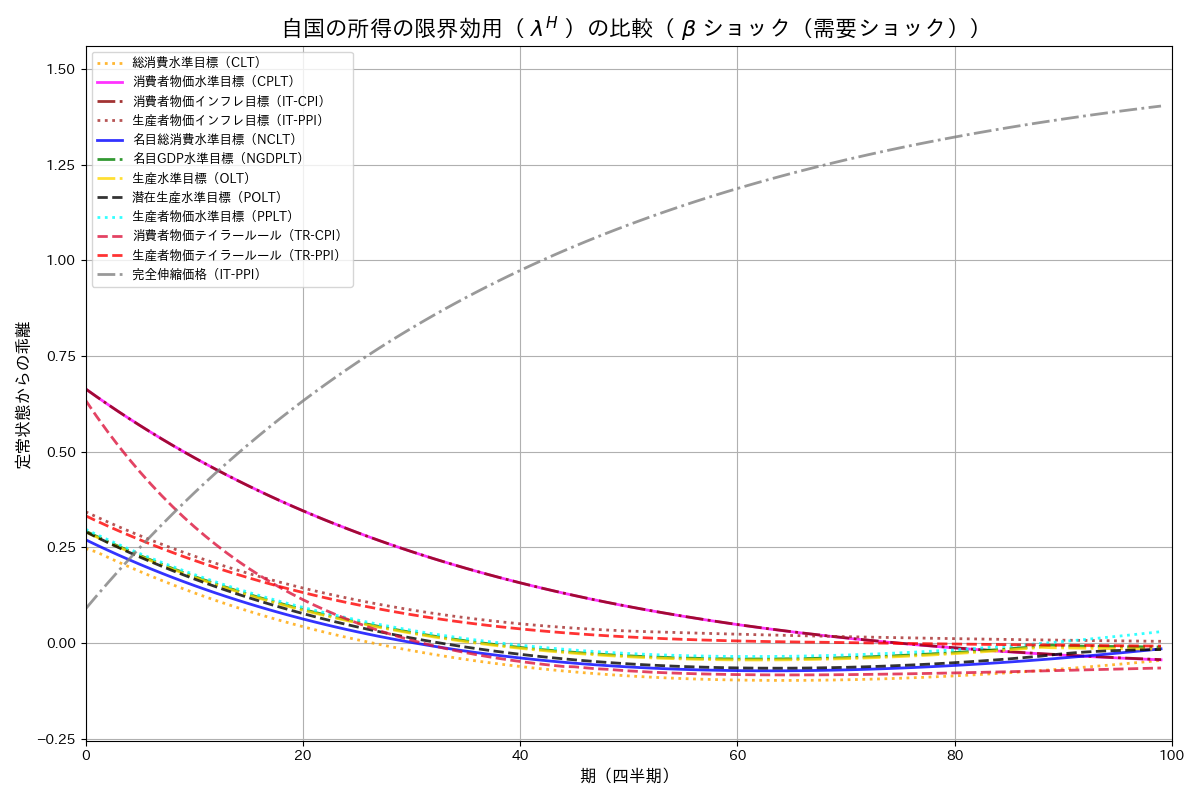
\includegraphics[width=0.9\textwidth]{comparison_graphs/beta_shock/beta_shock_lambda_H.png}
    \caption{自国の所得の限界効用\(\lambda^H\)}
    \label{fig:chapter5_beta_shock_asad_lambda_H}
\end{figure}
\begin{figure}[H]
    \centering
    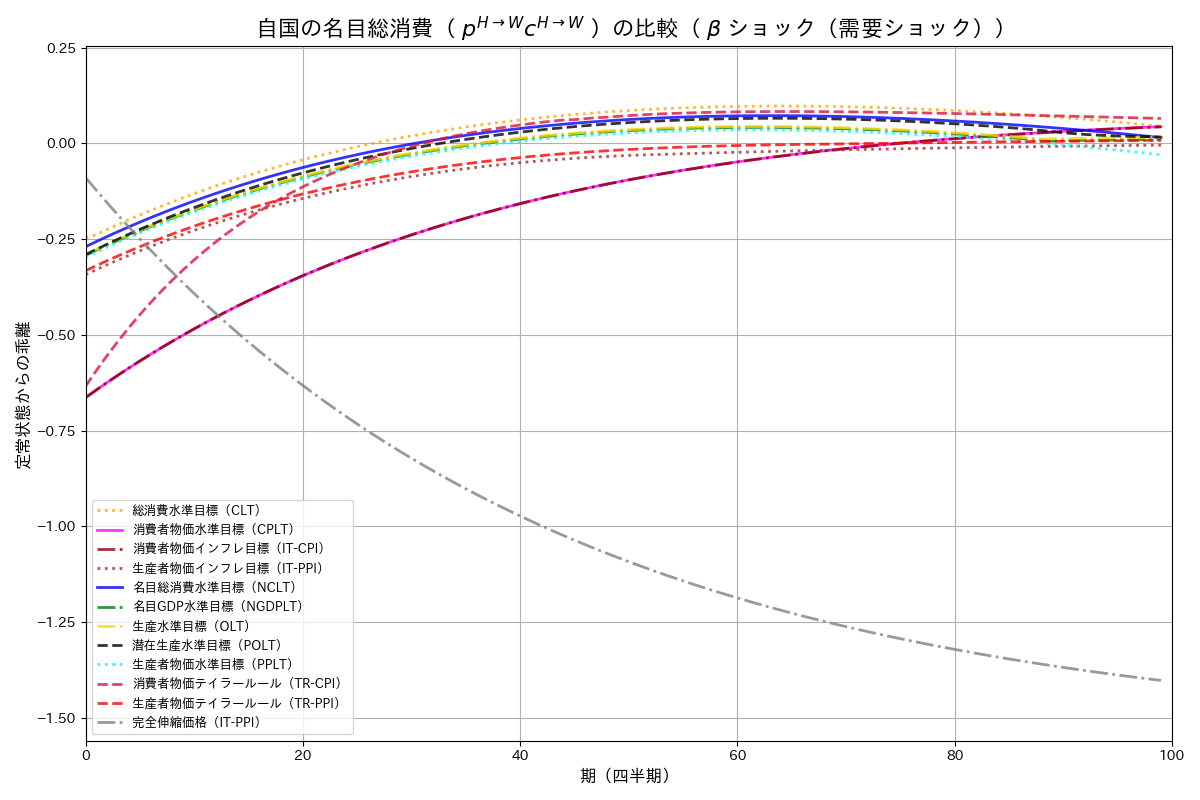
\includegraphics[width=0.9\textwidth]{comparison_graphs/beta_shock/beta_shock_p_H_W_c_H_W.png}
    \caption{自国の名目総消費\(p^{H\to W}c^{H\to W}\)}
    \label{fig:chapter5_beta_shock_asad_p_H_W_c_H_W}
\end{figure}
\begin{figure}[H]
    \centering
    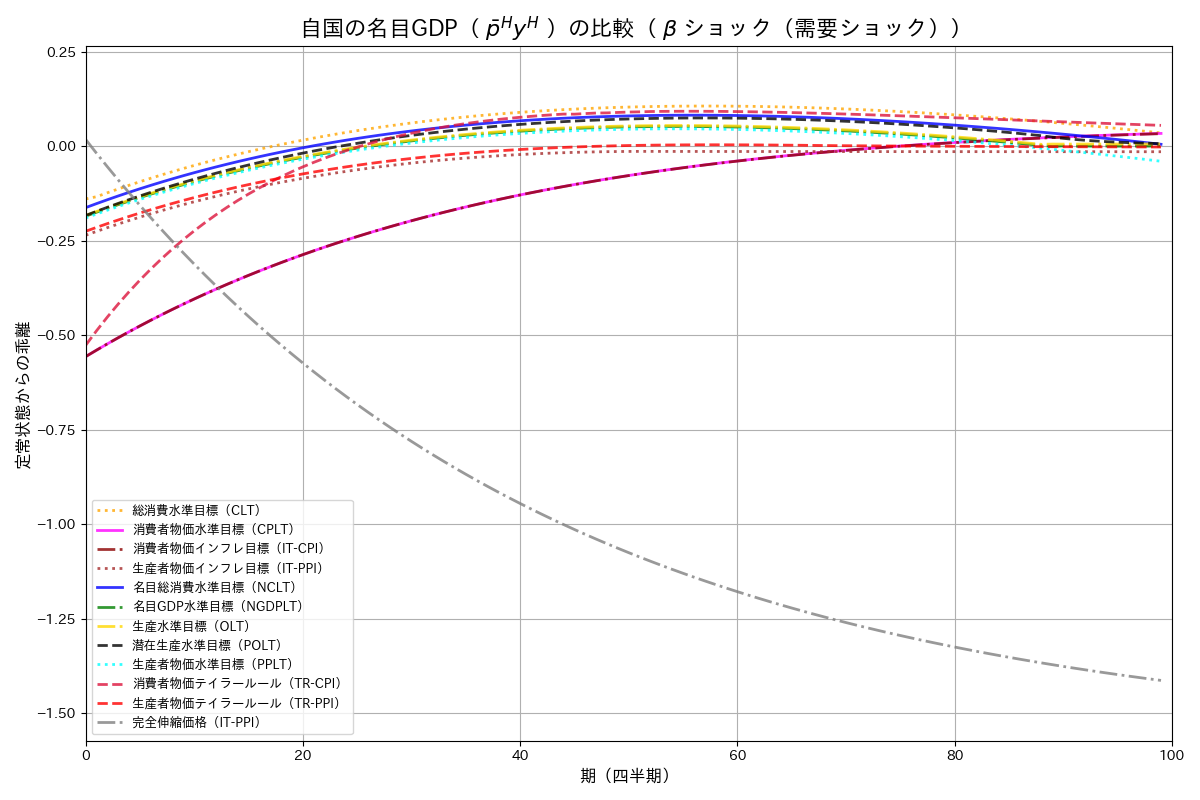
\includegraphics[width=0.9\textwidth]{comparison_graphs/beta_shock/beta_shock_p_H_bar_y_H.png}
    \caption{自国の名目GDP\(\bar{p}^Hy^H\)}
    \label{fig:chapter5_beta_shock_asad_p_H_bar_y_H}
\end{figure}
\begin{figure}[H]
    \centering
    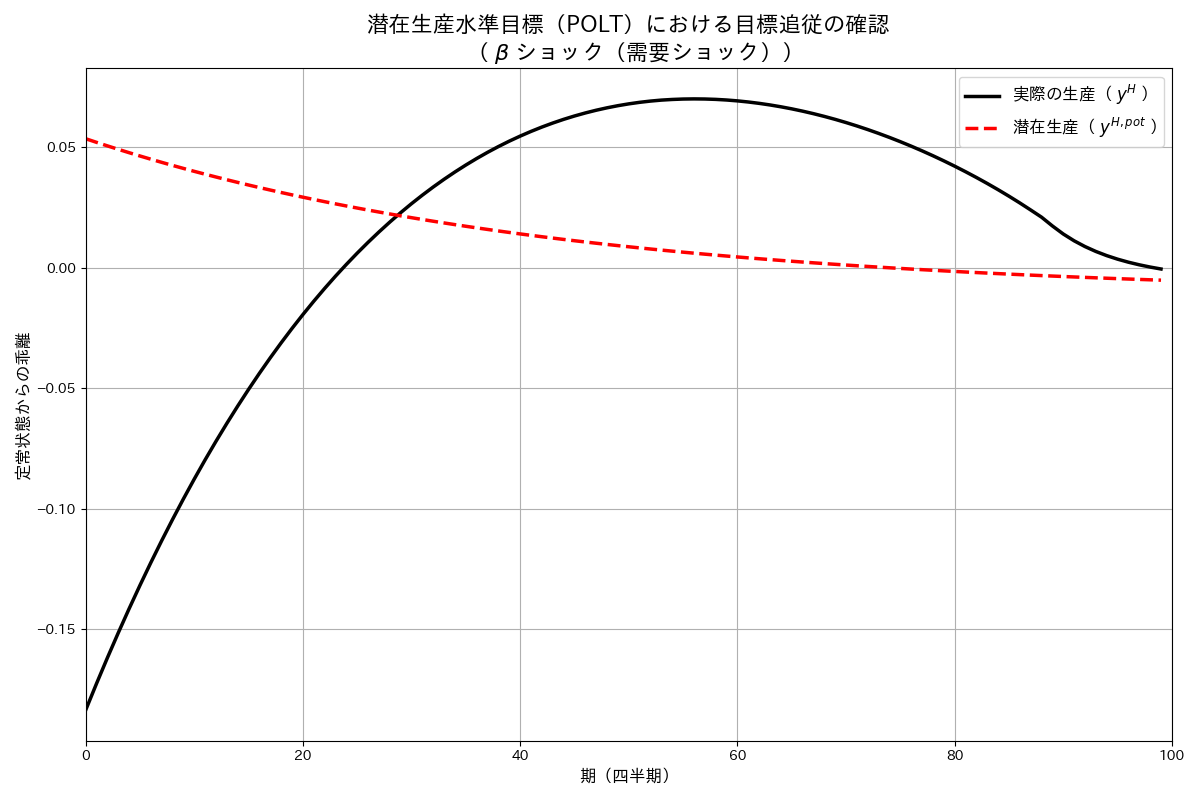
\includegraphics[width=0.9\textwidth]{comparison_graphs/beta_shock/beta_shock_polt_y_H_and_y_H_potential.png}
    \caption{自国の生産\(y^H\)と潜在生産\(y^{H,pot}\)潜在生産水準目標}
    \label{fig:chapter5_beta_shock_asad_y_H_potential}
\end{figure}
\begin{figure}[H]
    \centering
    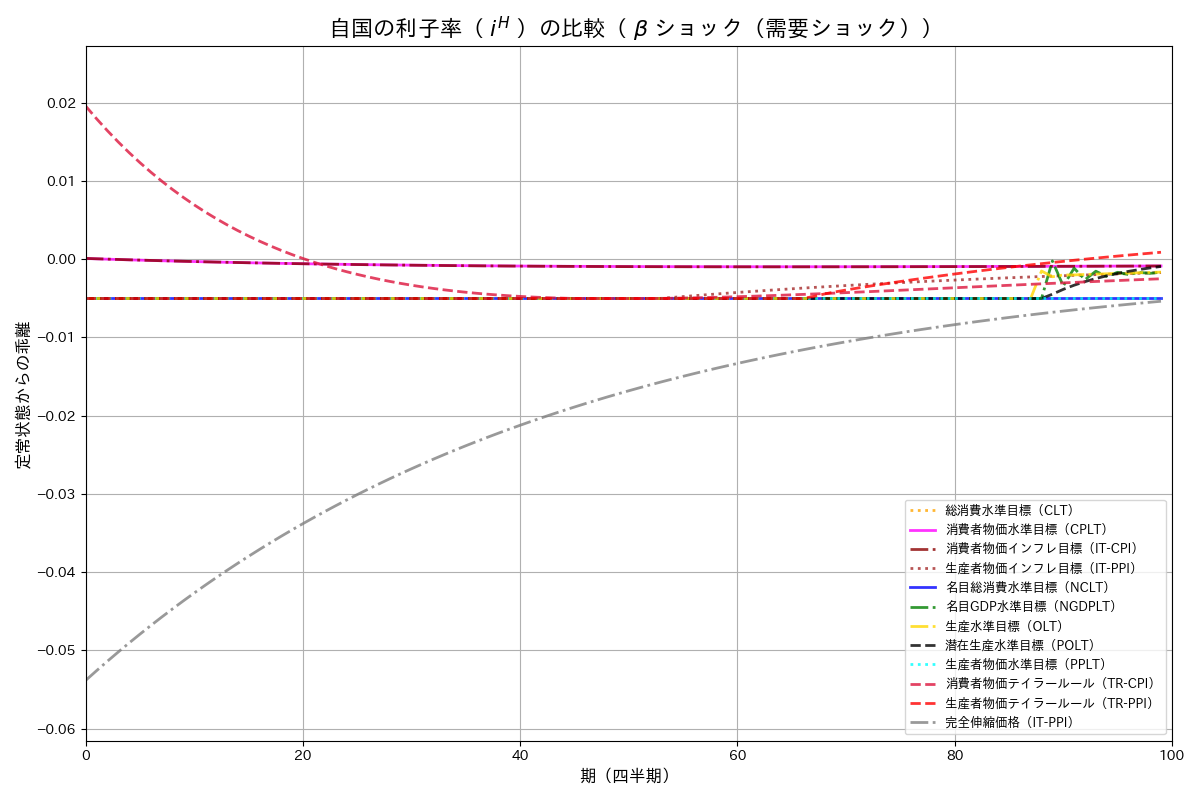
\includegraphics[width=0.9\textwidth]{comparison_graphs/beta_shock/beta_shock_i_H.png}
    \caption{自国の名目利子率\(i^H\)}
    \label{fig:chapter5_beta_shock_asad_i_H}
\end{figure}
\begin{figure}[H]
    \centering
    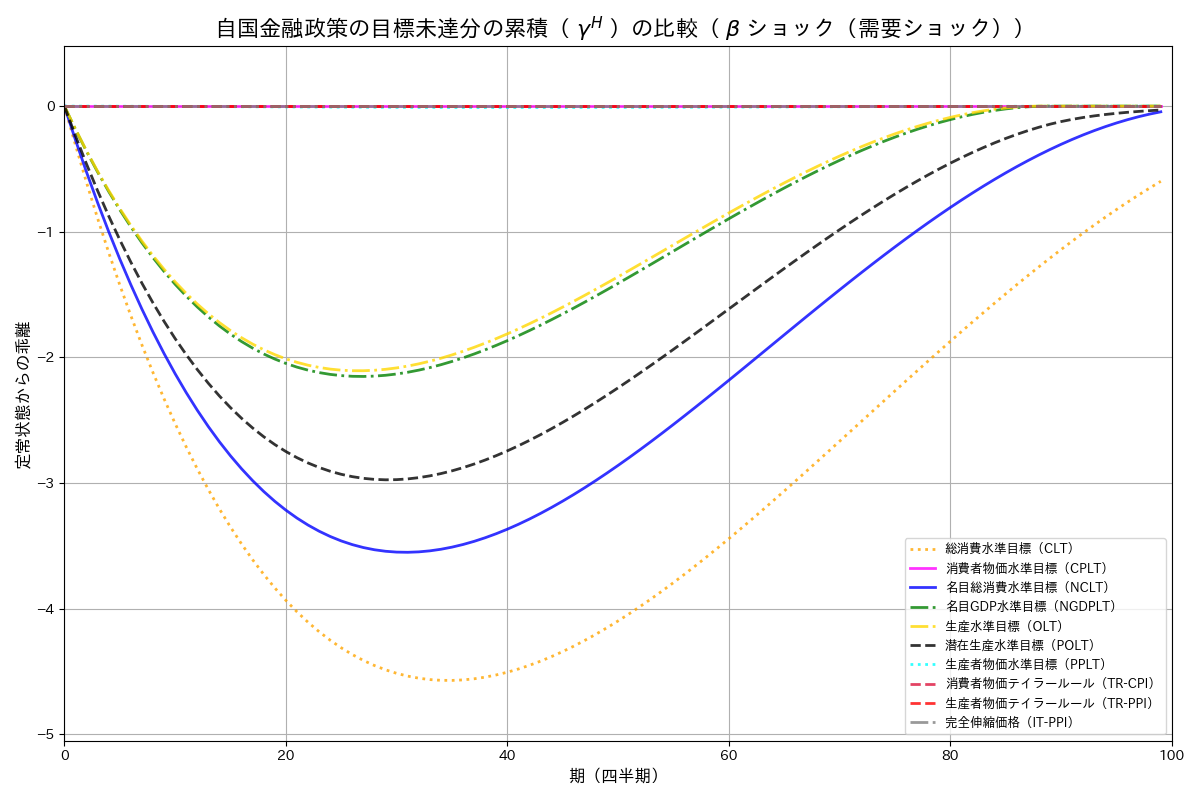
\includegraphics[width=0.9\textwidth]{comparison_graphs/beta_shock/beta_shock_gamma_H.png}
    \caption{自国の目標未達分の累積\(\gamma^H\)}
    \label{fig:chapter5_beta_shock_asad_gamma_H}
\end{figure}

\subsubsection{各政策の分析}
\label{sec:chapter5_beta_shock_asad_policies}
ここから各政策について、厚生\(W^H\)の落ち込みが小さい（評価が高い）順に、
AS-AD曲線などを用いた理論的分析をおこなう。
厚生\(W^H\)の式
\eqref{form:chapter5_beta_shock_welfare_W_H_substituted_eq}
によれば、その決定要因は以下の4つの変数であった。
\begin{enumerate}
    \item
    \label{itm:chapter5_beta_shock_asad_policies_c_H_W}
        \(c_t^{H \to W}\)：
        厚生\(W^H\)と正の相関がある。
    \item
    \label{itm:chapter5_beta_shock_asad_policies_y_H}
        \(y_t^H\)：
        厚生\(W^H\)と負の相関がある。
    \item
    \label{itm:chapter5_beta_shock_asad_policies_pi_H}
        \(\pi_t^H\)：
        定常状態からの乖離が厚生\(W^H\)と負の相関がある。
    \item
    \label{itm:chapter5_beta_shock_asad_policies_Delta_t_minus_1_H}
        \(\Delta_{t-1}^H\)：
        厚生\(W^H\)と負の相関がある。
\end{enumerate}
そこで、各政策が厚生\(W^H\)に予える影響を考えるために、
これらの4つの変数に与える影響について議論していくこととする。

\paragraph{名目総消費水準目標（NCLT）}
\label{sec:chapter5_beta_shock_asad_policies_nclt}
式
\eqref{form:chapter3_policies_monetary_home_nclt_i_H_eq}、
\eqref{form:chapter3_policies_monetary_home_nclt_gamma_H_eq}および
\eqref{form:chapter3_policies_monetary_home_clt_chi_H_eq}
により記述されたとおり、NCLTの式は以下のようであった。
\begin{align}
\label{form:chapter5_beta_shock_asad_policies_nclt_i_H_eq}
    i_t^H&=i_{ss}^H+\phi_{gap}^H(\log(p_t^{H\to W}c_t^{H\to W})-\log(\chi_t^H))+\phi_{level}^H\gamma_t^H \\
\label{form:chapter5_beta_shock_asad_policies_nclt_gamma_H_eq}
    \gamma_t^H&=\gamma_{t-1}^H+(\log(p_{t-1}^{H\to W}c_{t-1}^{H\to W})-\log(\chi_{t-1}^H)) \\
\label{form:chapter5_beta_shock_asad_policies_nclt_chi_H_eq}
    \log(\chi_t^H)-\log(\chi_{ss}^H)&=\rho_{\chi}^H\left(\log(\chi_{t-1}^H)-\log(\chi_{ss}^H)\right)+\varepsilon_t^{\chi,H}
\end{align}
ここで
\ref{sec:chapter3_policies_monetary_home_clt}
節より、\(\phi_{gap}^H, \phi_{level}^H\)は任意値のパラメータであった。
\begin{enumerate}
    \item 
    \label{itm:chapter5_beta_shock_asad_policies_nclt_c_H_W_detail}
        \(c_t^{H \to W}\)：
        NCLTの目標は名目総消費\(p_t^{H \to W}c_t^{H \to W}\)の維持である。
        図
        \ref{fig:chapter5_beta_shock_asad_p_H_W_c_H_W}
        に見られるとおり、需要ショック発生時、ジャンプ変数である消費\(c_t^{H \to W}\)は急落しようとするが、
        目標乖離を検知した中央銀行は名目利子率\(i_t^H\)を大幅に引き下げる。
        図
        \ref{fig:chapter5_beta_shock_insulation_e_slash_star}
        が示すとおり、この緩和に応答して名目為替レート\(e_t^{/*}\)は即座に減価（上昇）する。
        図
        \ref{fig:chapter5_beta_shock_asad_p_H_W}
        に見られるように、生産者物価指数（PPI）\(p_t^H, p_t^{F*}\)が硬直的な中、
        この名目為替レート\(e_t^{/*}\)の上昇が
        消費者物価指数（CPI）\(p_t^{H\to W}&=(p_t^H)^{\alpha^H}(e_t^{/*}p_t^{F*})^{1-\alpha^H}\)
        を押し上げる。
        この消費者物価指数（CPI）\(p_t^{H\to W}\)の上昇が
        名目総消費\(p_t^{H \to W}c_t^{H \to W}\)維持の枠組みで
        消費\(c_t^{H \to W}\)の減少分を相殺するため、図
        \ref{fig:chapter5_beta_shock_asad_c_H_W}
        のとおり消費\(c_t^{H \to W}\)は初期の落ち込みを最小限に留めている。
        また将来の名目総消費\(p_t^{H \to W}c_t^{H \to W}\)を保証する約束は
        所得の限界効用\(\lambda_t^H = 1/(p_t^{H \to W}c_t^{H \to W})\)を安定させる。
        これが将来の期待消費を潤沢にすると予想させる「期待のアンカー」となり、図
        \ref{fig:chapter5_beta_shock_asad_c_H_W}
        に見られるとおり、物価目標政策と比較して速やかな回復を実現している。
    \item 
    \label{itm:chapter5_beta_shock_asad_policies_nclt_y_H_detail}
        \(y_t^H\)：
        目標に「価格」が含まれていることで、
        実質変数の過剰な拡大に伴うインフレ圧力を自動的に検知して緩和にブレーキをかける。
        その結果、生産のオーバーシュートを小さく抑え、家計の過剰な労働を抑制することで厚生の悪化を防いでいる。
    \item 
    \label{itm:chapter5_beta_shock_asad_policies_nclt_pi_H_detail}
        \(\pi_t^H\)：
        名目支出目標が強力な名目アンカーとして機能する。
        将来の名目支出を保証するコミットメントが家計の期待インフレ率を安定させるため、
        実際のインフレ率の定常状態からの乖離そのものが低く抑え込まれ、フローの厚生損失を最小化している。
    \item 
    \label{itm:chapter5_beta_shock_asad_policies_nclt_Delta_t_minus_1_H_detail}
        \(\Delta_{t-1}^H\)：
        インフレ率の変動が全政策の中で最も低い水準で安定しているため、価格分散の蓄積も最小限である。
        この生産効率の悪化の抑制が、ストックの観点から厚生の維持に大きく貢献している。
\end{enumerate}
以上の分析から、NCLTがなぜ最高評価を得たのかが明らかになる。
NCLTは、素早い初動による消費の下支えを維持しつつも、
名目支出という枠組みを通じて「労働供給の過熱抑制」および「価格分散コストの抑制」を同時に達成しているのである。
この実質と名目のハイブリッドな安定化能力こそが、厚生を最大化させた本質的な要因である。

\paragraph{潜在生産水準目標（POLT）}
\label{sec:chapter5_beta_shock_asad_policies_polt}
POLTは実際の生産\(y_t^H\)と潜在生産\(y_t^{H,pot}\)との乖離（生産ギャップ）を目標とするルールであり、
次のように記述される。
\begin{equation}
\label{form:chapter5_beta_shock_polt_i_H_eq}
    i_{t,notional}^H=i_{ss}^H+\phi_{gap}^H(\ln y_t^H-\ln y_t^{H,pot})+\phi_{level}^H\gamma_t^H
\end{equation}
POLTの挙動において最も特徴的な点は、
目標である潜在生産自体が外生ショックに反応して動いている点である。
\begin{enumerate}
    \item
    \label{itm:chapter5_beta_shock_asad_policies_polt_potential}
        目標の動的変化と生産ギャップの拡大：
        図
        \ref{fig:chapter5_beta_shock_asad_y_H_potential}
        に示されるとおり、需要ショックが発生した直後、
        家計の貯蓄選好の高まりを反映して潜在生産\(y_t^{H,pot}\)は上昇する。
        一方で、実際の生産\(y_t^H\)は価格硬直性により需要の減退を直接受け、大幅に下落する。
        つまり、POLTでは目標（潜在生産）が上がり、実態（実際の生産）が下がるという二重の乖離が発生する。
        この巨大な生産ギャップの発生が、強力な緩和圧力を生む原動力となっている。
    \item
    \label{itm:chapter5_beta_shock_asad_policies_polt_zlb}
        最長のゼロ名目利子率継続と履歴依存性の役割：
        図
        \ref{fig:chapter5_beta_shock_asad_i_H}において、
        POLTは90期付近までゼロ名目利子率制約（ZLB）を継続しており、全政策の中で最も出口が遅い。
        式
        \eqref{form:chapter5_beta_shock_polt_i_H_eq}
        に含まれる累計乖離項\(\gamma_t^H\)が、初期に蓄積された巨大な負のギャップの記憶を保持しているため、
        過去の未達分を相殺するために生産が潜在水準を上回る「過熱状態」を長期間維持する必要が生じ、
        これがZLBの継続をもたらしている。
    \item
    \label{itm:chapter5_beta_shock_asad_policies_polt_drift}
        物価の著しい上昇ドリフト：
        図\ref{fig:chapter5_beta_shock_asad_p_H}において、
        国内財価格\(p_t^H\)は全政策で最も高い上昇を見せている。
        これは、上述の長期間にわたる過剰な金融緩和が将来の物価上昇期待を強力に押し上げ、
        水平なAS曲線
        \eqref{form:chapter5_asad_as_p_H_eq}
        を絶え間なく上方へシフトさせた結果である。
\end{enumerate}
以上の分析から、POLTは実体経済の過熱と物価の不安定化を招きやすい性質を持つことがわかる。
厚生$W^H$の観点からは、この過剰な労働供給と物価上昇に伴う価格分散コストがペナルティとなり、
実体経済を適度に制御しつつ名目アンカーを維持するNCLTに評価を譲る結果となっている。

\paragraph{生産水準目標（OLT）}
\label{sec:chapter5_beta_shock_asad_policies_olt}
OLTは実質生産\(y_t^H\)のみを目標とする政策ルールであり、次のように定義される。
\begin{equation}
\label{form:chapter5_beta_shock_olt_i_H_eq}
    i_{t,notional}^H=i_{ss}^H+\phi_{gap}^H(\ln y_t^H-\ln\chi^H)+\phi_{level}^H\gamma_t^H
\end{equation}
図\ref{fig:chapter5_beta_shock_asad_y_H}において、
OLTの生産パスは名目GDP水準目標（NGDPLT）とほぼ重なる軌道を描いている。
この類似性は、本稿の重要な設定である価格の硬直性（\(\kappa^H=0\)）に起因する。
NGDPLTが目標とする名目GDPにおいて、国内財価格\(p_t^H\)が極めて安定しているため、
名目値の変化は実質生産の変化とほぼ同義となり、結果としてOLTとNGDPLTは近似的に同一の政策として機能している。
OLTの動学特性における注目点は、物価の「上昇ドリフト」と「利子率の早期脱却」である。
\begin{enumerate}
    \item
    \label{itm:chapter5_beta_shock_asad_policies_olt_drift}
        名目アンカーの欠如による物価の推移：
        図\ref{fig:chapter5_beta_shock_asad_p_H}において、国内財価格\(p_t^H\)は定常状態から乖離し、
        右肩上がりの上昇傾向を見せる。需要ショック自体は本来物価に下落圧力をかけるが、
        OLTの下では中央銀行が生産の回復を最優先し、強力な金融緩和を継続する。
        OLTは物価水準を目標に含んでいないため、
        実体経済を回復させる過程で生じたインフレ期待を抑制する「ブレーキ」が働かない。
        その結果、AS曲線が将来の物価上昇期待\(E_t[\hat{p}_{t+1}^H]\)によって上方へシフトし続け、
        物価水準が定常状態から離れていくドリフト現象が生じている。
    \item
    \label{itm:chapter5_beta_shock_asad_policies_olt_exit}
        目標達成の早さと名目利子率の挙動：
        図\ref{fig:chapter5_beta_shock_asad_i_H}において、
        OLTは実質消費水準目標（CLT）に次いで早い時期にゼロ名目利子率制約（ZLB）から離脱している。
        これは、OLTが実質生産\(y_t^H\)を直接の目標としているため、ショックによって左方へシフトした
        AD曲線\eqref{form:chapter5_asad_ad_p_H_eq}を元の位置へ復元させる力が、
        目標変数に対して最もダイレクトに作用したためである。
\end{enumerate}
以上のとおり、OLTは生産の安定化において非常に強力な能力を発揮する。
しかし、目標に名目変数（物価や名目支出）を一切含まないため、
長期的な物価水準を一定に保つ能力（名目アンカー効果）を欠いている。この「物価の放任」が、
回復期において生産のオーバーシュートを招き、厚生$W^H$の評価をNCLT等に譲る要因となっている。

\paragraph{実質消費水準目標（CLT）}
\label{sec:chapter5_beta_shock_asad_policies_clt}
CLTは、物価等の名目変数ではなく、
家計の効用に直結する総消費指数\(c_t^{H\to W}\)そのものを目標とする政策ルールである。
\begin{equation}
\label{form:chapter5_beta_shock_clt_i_H_eq}
    i_{t,notional}^H=i_{ss}^H+\phi_{gap}^H(\ln c_t^{H\to W}-\ln\chi^H)+\phi_{level}^H\gamma_t^H
\end{equation}
図
\ref{fig:chapter5_beta_shock_asad_c_H_W}
および図
\ref{fig:chapter5_beta_shock_asad_i_H}
が示すとおり、
CLTは需要ショックに対して極めて迅速かつ強力な回復力を示している。
この「初動の速さ」と「復元の早さ」は目標である総消費指数\(c_t^{H\to W}\)が
\textbf{ジャンプ変数}であることに起因する。
\begin{enumerate}
    \item
    \label{itm:chapter5_beta_shock_asad_policies_clt_zlb}
        即時のZLB到達（初動の強さ）：
        前述のCPLTやPPLTが目標としていた「状態変数（物価）」とは異なり、
        実質消費\(c_t^{H\to W}\)はショックが発生した瞬間に将来の予測を織り込んで即座にジャンプする性質を持つ。
        需要ショックの直撃により消費が急落しようとした瞬間、
        式
        \eqref{form:chapter5_beta_shock_clt_i_H_eq}
        はその乖離を\(t=0\)の時点で直ちに検知する。
        その結果、図\ref{fig:chapter5_beta_shock_asad_i_H}のとおり、
        名目利子率\(i_t^H\)はショック発生と同時にゼロ名目利子率制約（ZLB）まで一気にジャンプする。
        この初動の速さが、AD曲線を即座に右上へと押し戻し、消費の初期落ち込みを最小限に留めている。
    \item
    \label{itm:chapter5_beta_shock_asad_policies_clt_expectation}
        期待を通じたAD曲線の復元：
        CLTの下では、中央銀行が「実質消費の水準」を維持することを家計にコミットしている。
        家計は、現在の消費が落ち込んでも中央銀行がそれを必ず元の水準へ戻すと確信するため、
        オイラー方程式における将来の所得の限界効用の期待値\(E_t[\lambda_{t+1}^H]\)が
        低下（将来の期待消費が潤沢になると予想）する。
        この期待のアンカーが、名目利子率のZLB継続と相まって、
        図
        \ref{fig:chapter5_beta_shock_asad_c_H_W}
        に見られるような急速なV字回復を実現させている。
    \item
    \label{itm:chapter5_beta_shock_asad_policies_clt_exit}
        最速のZLB出口（目標達成の早さ）：
        図\ref{fig:chapter5_beta_shock_asad_i_H}において、
        CLTは80期付近で他の政策よりも早くゼロ名目利子率を脱却している。
        これは、目標である実質消費\(c_t^{H\to W}\)が物価のような遅行指標（状態変数）ではなく、
        政策に対して最も感応度の高いジャンプ変数であるため、
        目標とする定常状態への復帰が早期に完了したことを意味する。
\end{enumerate}
以上の分析から、CLTは実体経済の痛みを直接検知し、
ジャンプ変数としての消費の性質を活かしてAD曲線に強力な復元力を与える、
極めて有効なショック緩和策であることが確認できる。
しかし、CLTは物価を目標に含んでいないため、物価の安定性やそれに伴う価格分散コストの抑制という観点では、
次に述べるNCLTに対して一歩譲ることになる。

\paragraph{名目GDP水準目標（NGDPLT）}
\label{sec:chapter5_beta_shock_asad_policies_ngdplt}
NGDPLTは国内財価格（PPI）\(\bar{p}_t^H\)と実質生産\(y_t^H\)の積を目標とするルールであり、
次のように定義される。
\begin{equation}
\label{form:chapter5_beta_shock_ngdplt_i_H_eq}
    i_{t,notional}^H=i_{ss}^H+\phi_{gap}^H(\ln\bar{p}_t^H+\ln y_t^H-\ln\chi^H)+\phi_{level}^H\gamma_t^H
\end{equation}
図\ref{fig:chapter5_beta_shock_asad_p_H_bar_y_H}等に示されるとおり、
NGDPLTはNCLTやCLTと並んで強力な回復力を示すが、それらと比較して「オーバーシュートが小さく、
定常状態への収束が早い」という穏やかな動学特性を持つ。
この差異は、目標に含まれる変数の構成、特に「物価指数の範囲」と「実数項の定義」の違いに由来する。
\begin{enumerate}
    \item
    \label{itm:chapter5_beta_shock_asad_policies_ngdplt_sensitivity}
        目標変数の感度の差：
        NCLTが目標とする名目消費には、
        ジャンプ変数である為替レート\(e^{/*}\)がCPIを通じて直接含まれている。
        一方、NGDPLTの目標である名目GDP（\(\bar{p}_t^Hy_t^H\)）に含まれる国内価格は、
        為替の影響を直接受けない純粋な状態変数である。
        このため、NGDPLTはNCLTに比べてショック直後の目標の変動が抑制され、
        それが政策利子率の早期脱却（図\ref{fig:chapter5_beta_shock_asad_i_H}）と、
        復興期における景気過熱（オーバーシュート）の回避につながっている。
    \item
    \label{itm:chapter5_beta_shock_asad_policies_ngdplt_cpi}
        消費者物価指数の乖離に関するパラドックス：
        図\ref{fig:chapter5_beta_shock_asad_p_H_W}において、
        NCLTの方がNGDPLTよりも消費者物価指数の定常状態からのプラスジャンプが大きくなっている。
        これは、NCLTが「CPIを含む名目支出」の維持を至上命題としているため、
        需要ショックによる実質消費の減少を相殺すべく、大胆に名目利子率を下げて為替を減価させ、
        CPIを強く押し上げている結果である。
        対してNGDPLTは国内指標を重視するため、為替を介した輸入物価の押し上げには相対的に消極的であり、
        その結果としてCPIのジャンプ幅が小さく留まっている。
    \item
    \label{itm:chapter5_beta_shock_asad_policies_ngdplt_convergence}
        収束の早さと安定性：
        NGDPLTが全政策中で最も早く定常状態へ収束している点は注目に値する。
        これは、国内生産\(y_t^H\)を目標に据えることで、
        国内の需給バランスを直接的にアンカーしているためである。
        消費\(c_t^{H\to W}\)は異時点間の最適化によって大きく変動しやすい性質を持つが、
        生産\(y_t^H\)は経済全体の安定化を図る上では名目GDPを指標とする方が、
        動学的な揺れを最小限に抑えやすい傾向がある。
\end{enumerate}
以上の比較分析から、NGDPLTはNCLTほどの需要回復力は持たないものの、
実体経済の過熱を抑制し、最も安定的かつ早期に経済を平時へと帰還させる能力に長けていると言える。
この性質が、厚生$W^H$評価においてNCLTに次ぐ高い評価を支える要因となっている。

\paragraph{生産者物価水準目標（PPLT）}
\label{sec:chapter5_beta_shock_asad_policies_pplt}
PPLTは自国財価格指数\(p_t^H\)のみを目標とする政策であり、その式は以下のように記述される。
\begin{equation}
\label{form:chapter5_beta_shock_pplt_i_H_eq}
    i_{t,notional}^H=i_{ss}^H+\phi_{gap}^H(\ln p_t^H-\ln\chi^H)+\phi_{level}^H\gamma_t^H
\end{equation}
PPLTにおいて特筆すべきは、図\ref{fig:chapter5_beta_shock_asad_i_H}に示されるとおり、
名目利子率\(i_t^H\)がショック直後の\(t=0\)においてジャンプせず定常状態から始動し、
その後も他の緩和的な政策群（NCLT等）とは対照的に、
ゼロ名目利子率制約（ZLB）に達するほどの強力な緩和を行っていない点である。
この不十分な初動の背景には、目標変数の「純粋な状態変数性」がある。
PPLTが凝視する自国財価格\(p_t^H\)は、為替の影響すら受けない純粋な\textbf{状態変数}である。
本モデルのように価格粘着性が極めて高い設定下では、物価はショック直後には一切動かず、
時間の経過とともに極めて緩やかに低下していく。
式\eqref{form:chapter5_beta_shock_pplt_i_H_eq}にもとづけば、
目標である\(p_t^H\)が\(t=0\)で動かない以上、中央銀行はショックの直撃を検知できず、
名目利子率を引き下げる根拠を持たない。
この「初動の遅れ」は、AD曲線の復元において決定的な足かせとなる。
\begin{enumerate}
    \item
    \label{itm:chapter5_beta_shock_asad_policies_pplt_exchange_rate}
        為替の不在：CPLTでは為替レート\(e^{/*}\)を操作することでCPIの数値を「無理やり」固定できたが、
        PPLTの目標には為替が含まれない。そのため、名目利子率操作が為替を動かしても、
        それが直接目標の安定に寄与せず、むしろ物価が実際に下落し始めるのを待つしかない。
    \item
    \label{itm:chapter5_beta_shock_asad_policies_pplt_demand}
        需要の放置：オイラー方程式において、名目利子率\(i_t^H\)が十分に低下せず、
        かつ将来の価格上昇へのコミットメントも物価が動き出すまで発動しないため、
        AD曲線は左方に沈んだままとなる。
        これが、図\ref{fig:chapter5_beta_shock_asad_y_H}等で示される深刻な生産の落ち込みを招く。
\end{enumerate}
図\ref{fig:chapter5_beta_shock_asad_p_H}が示すとおり、
PPLTは「水準目標」としての履歴依存性を持つため、
長期的には物価を定常状態へ戻す能力において全政策中で最も高い精度を見せる。
しかし、価格という「極めて動きの遅い敵」が動き出すのを待ってからしか反応できないという性質上、
ショック初期の数年間においては実体経済を深刻な不況にさらすこととなる。
厚生$W^H$の観点からは、長期的な物価の正確な復元よりも、初動でのジャンプによる需要の下支えが重要であり、
PPLTがCPLT同様に低い評価に留まる理由はここにある。

\paragraph{消費者物価水準目標（CPLT）}
\label{sec:chapter5_beta_shock_asad_policies_cplt}
CPLTは図
\ref{fig:chapter5_beta_shock_asad_p_H_W}
において消費者物価指数\(p_t^{H\to W}\)を定常状態の水準に固定している。
この極めて高い制御性は目標を構成する各変数の動学的な性質による。
まず目標である消費者物価指数\(p_t^{H\to W}\)は定義式
\eqref{form:chapter3_households_stage1b_cpi_descriptions_p_H_W_eq}
において外国財価格指数\(p_t^F=e_t^{/*}p_t^{F*}\)を代入することにより
次のように表せる。
\begin{equation}
\label{form:chapter5_beta_shock_cplt_p_H_W_eq}
    p_t^{H\to W}=(p_t^H)^{\alpha^H}(e_t^{/*}p_t^{F*})^{1-\alpha^H}
\end{equation}
ここで国内財価格指数\(p_t^H\)および外国財価格指数\(p_t^{F*}\)は
前期の経済において決まる\textbf{状態変数}であり、
ショックが発生した\(t=0\)においては定常状態から動くことはない。
一方で、名目為替レート\(e_t^{/*}\)は以下の外国通貨建てリスクフリー債券に関するオイラー方程式に従う
\textbf{ジャンプ変数}であった。
\begin{equation}
\label{form:chapter5_beta_shock_cplt_lambda_H_i_F_eq}
    \lambda_t^He_t^{/*}=(1+i_t^F)\beta_t^H\operatorname{E}_t[\lambda_{t+1}^He_{t+1}^{/*}]
\end{equation}
さらに、この式に含まれる所得の限界効用\(\lambda_t^H\)は以下の自国コンティンジェント債券に関するオイラー方程式に従う。
\begin{equation}
\label{form:chapter5_beta_shock_cplt_lambda_H_i_H_eq}
    \lambda_t^H=\beta_t^H(1+i_t^H)\operatorname{E}_t[\lambda_{t+1}^H]
\end{equation}
これら2つの式からわかるように、中央銀行による名目利子率\(i_t^H\)の操作は式
\eqref{form:chapter5_beta_shock_cplt_lambda_H_i_H_eq}
を通じて所得の限界効用\(\lambda_t^H\)を即座に変化させ、さらに式
\eqref{form:chapter5_beta_shock_cplt_lambda_H_i_F_eq}
を通じて為替レート\(e_t^{/*}\)もそれに即座に反応する性質を持つ。
時間が経過し、状態変数である\(p_t^H\)や\(p_t^{F*}\)が低下し始めると、
中央銀行はそれを検知して名目利子率操作をおこなう。
このとき、反応の遅い物価の下落圧力に対し、反応の極めて速い為替レートを対置させることで、
式
\eqref{form:chapter5_beta_shock_cplt_p_H_W_eq}
の値を常に一定に保つような精密な相殺が可能となる。
しかしこの制御の容易さは実体経済の安定を意味しない。
AD曲線を右上へ復元させ需要の蒸発を防ぐためには
ショック直後の\(t=0\)における大胆な名目利子率低下と為替のジャンプが必要である。
物価という遅行指標のみを目標とするCPLTは、
初動において「まだ物価は動いていない」と判断して緩和シグナルを発することができない。
結果として、物価の数字上の安定と引き換えに、
ジャンプ変数である実質消費\(c_t^{H\to W}\)の深刻な急落を放置することになり、
厚生$W^H$を大きく損なう結果となっている。

\paragraph{インフレ目標（IT）}
\label{sec:chapter5_beta_shock_asad_policies_it}
図\ref{fig:chapter5_beta_shock_asad_pi_H}が示すとおり、
IT下でのインフレ率は初期に全政策の中で最も大きく下落している。
「物価の安定（インフレの維持）」を掲げる政策が、皮肉にも最も深刻なデフレを許容してしまった理由は、
本モデルの動学的な構造から次のように説明できる。
まず、自国財のグロス・インフレ率\(\pi_t^H\)の定義を確認する。
自国の全企業が同一の価格設定を行う本モデルの設定下では、インフレ率は自国財価格を用いて次のように記述される。
\begin{equation}
\label{form:chapter5_beta_shock_it_pi_def}
    \ln\pi_t^H=\ln p_t^H-\ln p_{t-1}^H
\end{equation}
図\ref{fig:chapter5_beta_shock_asad_pi_H}においてインフレ率の絶対的な変動幅が極めて小さいのは、
価格粘着性が極端に高い（\(\xi^H=0.99\)）ために、
その原資である国内物価指数\(p_t^H\)の動き自体が抑制されているためである。
ITにおいてインフレ率が全政策で最も低くなった原因は、水準目標が持つ「履歴依存性」の欠如にある。
AS曲線（フィリップス曲線）にもとづけば、
現在のインフレ率は将来のインフレ期待\(E_t[\pi_{t+1}^H]\)に強く依存する。
\begin{enumerate}
    \item
    \label{itm:chapter5_beta_shock_asad_policies_it_expectation}
        期待の崩壊：NCLTやPPLTのような水準目標は、ショックで物価が下がれば、将来それを埋め合わせるために「目標を上回るインフレ」を生成することを約束する。しかし、ITは過去の未達分を考慮しないため、家計は「物価は下がったままで、将来も中央銀行が物価を押し戻すことはない」と予想する。この期待インフレ率の低下が、現在のインフレ率をさらに押し下げるという負のスパイラルを生んでいる。
    \item
    \label{itm:chapter5_beta_shock_asad_policies_it_reaction}
        不十分な名目利子率反応：ITの政策は現在のインフレ率のみに反応する。
    \begin{equation}
    \label{form:chapter5_beta_shock_it_i_H_eq}
        i_{t,notional}^H=i_{ss}^H+\phi_\pi^H(\ln\pi_t^H-\ln\pi_{ss}^H)
    \end{equation}
    図
    \ref{fig:chapter5_beta_shock_asad_i_H}
    が示すとおり、IT下の名目利子率は初期にわずかに低下するものの、
    水準目標群のようにゼロ金利に張り付くほどの大胆な緩和を見せない。
    これは、目標であるインフレ率が水準に比べて変化率として小さく見えるため、
    中央銀行が危機の深刻さを過小評価してしまうからである。
\end{enumerate}
最終的にインフレ率が定常状態に向かって回復しているのは、
需要ショック\(\beta_t^H\)自体が時間とともに減衰するという外生的な要因によるものであり、政策の力ではない。
オイラー方程式を通じて将来の物価上昇をコミットできないITは、実質利子率の高止まりを許容し、
AD曲線
\eqref{form:chapter5_asad_ad_p_H_eq}
を左方に放置し続ける。
これが、厚生$W^H$を全政策で最も悪化させた数理的な帰結である。

\subsection{厚生の決定要因：価格分散と実体経済のトレードオフ}
\label{sec:chapter5_beta_shock_analysis}
本節の締めくくりとして、なぜ名目総消費水準目標(NCLT)が厚生において最高評価を得たのかを、
図\ref{fig:chapter5_beta_shock_asad_delta_H}の価格分散（\(\Delta^H\)）の視点を交えて総括する。
各政策のパフォーマンスは、以下の3つの要因のバランスによって決定されている。
\begin{enumerate}
    \item
    \label{itm:chapter5_beta_shock_analysis_jump}
        \textbf{初動の速さ（ジャンプ変数の活用）}：
        ITやCPLT,PPLTといった「ショックを緩和できない政策群」は、目標が状態変数（物価）のみ、
        あるいは期待のアンカーを欠いているため、ショック直後の\(t=0\)で名目利子率を十分に下げられない。
        これに対し、NCLTやCLTはジャンプ変数である実質消費を目標に含むことで、
        ショックと同時に名目利子率をZLBまでジャンプさせ、不況の深刻化を未然に防いでいる。
    \item
    \label{itm:chapter5_beta_shock_analysis_anchor}
        \textbf{名目アンカーによる物価ドリフトの抑制}：
        CLT,OLT,POLTといった実質変数のみを追う政策は、実体経済を強力に回復させる一方で、
        物価水準を定常状態へ戻す力が弱い。
        図
        \ref{fig:chapter5_beta_shock_asad_p_H}
        に見られる物価の上昇ドリフトは、長期的には経済の不確実性を高める要因となる。
        NCLTは名目支出を目標とすることで、不況期には強力な緩和を行いながらも、
        回復期には物価上昇を検知して適切にブレーキをかけ、物価を定常状態へと収束させている。
    \item
    \label{itm:chapter5_beta_shock_analysis_delta}
        \textbf{価格分散コスト(\(\Delta^H\))の最小化}：
        厚生を最も大きく損なう要因の一つが、インフレ率の変動に伴う価格分散である。
        図
        \ref{fig:chapter5_beta_shock_asad_delta_H}
        を見ると、
        IT（インフレ目標）が突出して高い価格分散を記録している。
        これはITが水準目標を持たないためにデフレ期待のアンカーに失敗し、
        物価の大きな下落とその後の揺り戻しを許容してしまったためである。
        対照的に、NCLTは図
        \ref{fig:chapter5_beta_shock_asad_delta_H}
        において最も低い水準で\(\Delta^H\)を安定させている。
        これは、将来の名目支出を保証することで期待インフレ率を一定に保ち、
        実際のインフレ率の変動幅を最小限に抑え込んだ結果である。
\end{enumerate}
以上の分析から、NCLTの優位性は、(1)消費というジャンプ変数を検知する「鋭い初動」、
(2)名目支出という枠組みによる「物価の安定（名目アンカー）」、
および(3)それらがもたらす「価格分散コストの抑制」という3点を、
単一のルールで最も高次元にバランスさせた点にあると結論付けられる。